\documentclass[preprint,12pt,authoryear]{elsarticle}

\usepackage[utf8]{inputenc}
\usepackage{amsmath}
\usepackage{booktabs}
\usepackage{graphicx}
\usepackage{natbib}
\usepackage{url}
\usepackage{xurl}
\usepackage{microtype}
\usepackage{siunitx}
\usepackage{array}
\usepackage{lmodern}

\journal{Environmental Modelling \& Software}

\begin{document}

\begin{frontmatter}
\title{Discard or reconstruct? A leakage-safe benchmark of gap handling for annual heat extremes and their trends in river-temperature archives}

\author[aff1]{[AUTHOR TO CONFIRM]\corref{cor1}}
\affiliation[aff1]{organization={[AFFILIATIONS TO CONFIRM]}}
\cortext[cor1]{Corresponding author: [AUTHOR TO CONFIRM, email address]}


\begin{abstract}
Long-term analyses of river temperature commonly discard incomplete years, but how this screening affects annual heat extremes and their trends has rarely been quantified against reconstruction. We present an open, leakage-safe benchmark that jointly masks multi-year station archives, reconstructs annual maxima of 30-day mean water temperature (H30), and scores finite-record trends at 41 European and US stations (median 14 reference years). Fully observed 30-day windows in incomplete years exceeded complete-year records at 20 of 96 long-record stations. Under realistic gap calendars, screening and reconstruction inflated total trend uncertainty by 1.8\% and 0.5\%; under severe 30--90-day controlled gaps, by 21.5\% and 3.7\% (trend RMSE 0.446 versus 0.170 $^{\circ}$C per decade). Interval undercoverage concentrated in air-temperature-based reconstructions in Bavaria, and no method won universally: calendar-aware year selection helped at fixed year counts but less than reconstruction. The primitives and a dated benchmark layer are released as gapbench 1.3.0; the study pipeline is in the public compendium, with an archival DOI pending.

\end{abstract}

\begin{keyword}
river temperature \sep heat extremes \sep missing data \sep gap handling \sep trend uncertainty \sep open-source software
\end{keyword}

\begin{highlights}
\input{highlights.txt}
\end{highlights}
\end{frontmatter}

\IfFileExists{body.tex}{%
  \section{Introduction}

River water temperature integrates atmospheric forcing, catchment storage, and channel geometry, and its extremes structure thermal habitat and water-quality management \citep{webb2008,mohseni1998}. Air temperature is the dominant seasonal control, but the residual response depends on flow and heat capacity \citep{vanvliet2011,toffolon2015}, groundwater inflow \citep{johnson2021,gallice2015}, snow and ice melt \citep{isaak2012,arismendi2014}, lake and reservoir regulation \citep{beaufort2022,diaz2025}, and riparian shading. These controls make river temperature a distributed, non-stationary response rather than a deterministic function of air temperature, and process-based and machine-learning models can represent parts of it \citep{feigl2021,rahmani2021}. They also determine what a monitoring gap hides: a hot spell may coincide with low flow, a reservoir release, a groundwater-dominated reach, or a shaded headwater, and the same air-temperature anomaly can produce different water-temperature peaks in each setting.

Long summer gaps are not random. Low flows can expose sensors; heatwaves concentrate maintenance; storms and floods damage equipment; ice and access constrain winter service. A gap that removes a hot spell removes both an annual extreme and the leverage that year would have had on a multi-decade slope. The usual response is completeness screening: discard incomplete station-years, or discard stations that do not meet a completeness threshold. The cost can be large. In the 2,700 station-year observation panel used here, strict complete-year selection admits 2,139 years and discards 561, of which 545 still contain a fully observed 30-day window; a station-specific warm-season rule admits 2,634 years and excludes 66, of which 50 still contain such a window. Large syntheses face the same filter: \citet{hare2021} retained 197 of 1,424 stations after requiring more than 14 complete years. Screening is therefore a data-use decision with scientific consequences, not a neutral quality control.

Prior work has quantified parts of this problem. \citet{johnson2021} evaluated missing intervals and imputation for annual mean, phase and amplitude, and found river-dependent limitations. \citet{beaufort2022} built a multiyear thermal-peak metric from heterogeneous summer observations with climate correction. \citet{isaak2012} used reconstructed records to estimate long-term thermal trends, and \citet{diaz2025} evaluated process-stratified machine-learning predictions of daily temperature with coverage by groundwater, reservoir and thermal-discharge setting. None of these studies compares screening and reconstruction on the same finite-record annual heat extreme, with whole multiyear archives degraded jointly and the slope scored against a fixed reference-year set. The distinction matters because year loss and reconstruction error can offset or reinforce each other, and because a daily-error metric need not preserve the annual maximum or its trend.

We therefore ask three questions. First, what observed heat information does each completeness rule retain or discard? Second, how do the retained year set and annual reconstruction error combine in a finite-record slope? Third, under which visible information conditions does annual recovery fail? The answers are conditional on a long-complete cohort, not a random sample of rivers, and they concern a finite-record target rather than an identified climate-process trend.

The annual maximum 30-day mean water temperature ($\mathrm{H30}$) is a sustained-heat summary, not an ecological standard. A seven-day window (H7) is a different target, and we report an H7 refit only as a robustness check rather than substituting it for $\mathrm{H30}$.

Our contributions are three. (i) We introduce a leakage-safe, joint whole-archive benchmark: multiyear station records are masked together, hidden values never enter the local fit, year selection never sees temperature, and screening and reconstruction are scored on the same reference-year set. The benchmark separates year-set error, reconstruction error, and their cross term. (ii) We release \texttt{gapbench} 1.3.0, a small MIT-licensed NumPy-only Python library that exposes the reusable primitives (observed-window bounds, finite-record slopes, calendar-only year selection, slope-error decomposition, group-disjoint splits, archive masking) and a dated benchmark layer (annual H30 with observed lower bounds, a reproducible gap generator, dependency-free baselines, and a runner for user-supplied reconstructors) with tests, documentation and a synthetic quickstart. (iii) We report a quantitative case study of 41 European and US stations in 17 connected groups, with 805 controlled-gap archives and 818 empirical calendars, and we identify failure boundaries: severe controlled (mostly warm-season) gaps favor reconstruction; realistic gap calendars leave screening and reconstruction differences below the trend's own sampling error; fixed-count calendar selection helps but does not match all-year recovery; and air-only reconstruction without local water information fails on hidden peaks in regulated Bavarian rivers. We treat the observed-window result as a data-use principle, not as a separate contribution, and we do not claim a causal low-flow mechanism.

\textbf{Related literature and positioning.} Our evaluation framing borrows the iterative development-and-evaluation perspective \citep{jakeman2006} and the performance-characterization framework \citep{bennett2013}: the question is what a model is for, which errors matter, and how performance should be reported, not whether a single fit statistic is high. The software release follows reproducibility and FAIR-software arguments \citep{hutton2016,barker2022}, but we do not claim a full FAIR assessment or an executable workflow. River-temperature trend analyses \citep{orr2015} and reconstruction at unmonitored sites \citep{zwart2023} share our concern with screening and spatial transfer, but they use longer records, different targets and different validation designs. Regulation and catchment attributes are available from global dam and reach datasets \citep{lehner2011,linke2019} and from large-sample Swiss, German and Central European collections \citep{hoge2023,loritz2024,klingler2021}; our roster does not support a uniform covariate analysis. We borrow framing and context from these lines of work, not their models or validation designs.

\section{Framework}

\subsection{Joint masking and separation of fitting from evaluation}

The benchmark treats a station archive as a multiyear daily series and degrades it jointly, rather than masking isolated days. For station $i$, repetition $r$ and gap setting $g$, an archive $a=(i,r,g)$ is degraded year by year: each analysis year is masked independently with probability 0.35 following a seven-year fully observed burn-in, and the forward analysis starts in 2010, so the median archive has 36\% of its analysis years masked and no archive is masked in every year. In the empirical-calendar family, a year-specific calendar is instead copied from the observed archive. All masks are drawn before any model is fitted. The hidden water-temperature values are stored only for scoring. A local fit may use visible gap geometry, a training-period climatological peak, local water history, air temperature, and available neighboring stations; it may not use the hidden values, the true peak location, or the evaluated annual outcome. Twenty source repetitions redraw masks and group-role composition; they describe variability within the archive, not twenty independent climates. Figure~\ref{fig:architecture} separates the observation-only, annual-recovery and whole-archive evidence layers.

Fitting and evaluation are separated by connected groups. A connected group is a set of stations linked by the same river network or record family; it is the cluster unit for calibration and resampling. Group-disjoint splitting follows the cross-validation guidance for hierarchically and spatially structured data \citep{roberts2017}: every record from a connected group is assigned to one side of a split. Random record-level splitting would instead leak information across correlated stations of the same river. Source-role calibration estimates empirical offsets on groups disjoint from the target group. In the forward design, the HUC17 estimator role and the NVE interval-calibration role retain other same-region groups; the strict-region sensitivity removes them. This is a deliberate compromise between statistical separation and data availability, and we report it as a limitation rather than as a clean regional holdout.

The target is defined on a station-specific reference-year set $Y_i$, the complete years available under the evaluation design. $Y_i$ need not be contiguous, and years outside it are not imputed as part of the target. For $y\in Y_i$, write $x_{iy}=(y-\bar y_{Y_i})/10$ and $w_{iy}=x_{iy}/\sum_{y'\in Y_i}x_{iy'}^2$. The finite-record slope is
\begin{equation}
\beta_i=\sum_{y\in Y_i}w_{iy}\,\mathrm{H30}_{iy}.
\label{eq:beta}
\end{equation}
Restoring all supported years means restoring masked years within $Y_i$, not completing the surrounding calendar. All masks, retention rules and scores act on the same $Y_i$.

Procedure~1 summarizes the loop. Step~2 is the only step that sees hidden values, and it is an evaluation step. Step~4 is outcome-blind by construction: the selection function receives calendar years, complete-year labels, the objective and the target count, but no temperature, prediction or error.

\begin{center}
\fbox{\begin{minipage}{0.96\textwidth}
\small
\textbf{Procedure 1. Joint whole-archive benchmark.}
\begin{enumerate}
\item Fix station $i$, reference-year set $Y_i$, and archive $a=(i,r,g)$.
\item Mask a contiguous segment, or apply an empirical calendar, to every year in the archive jointly; store the hidden values for scoring only.
\item Fit or apply the annual recovery model using visible data and source groups disjoint from the target group.
\item Recover $\mathrm{H30}_y$ or the observed bound $L_y$ for every year; select retained years with a calendar-only rule.
\item Fit the finite-record slope on the selected set; score it against $\beta_i$ and decompose the error into $S$, $R$ and $E=S+R$.
\item Repeat over masks and repetitions; resample connected groups for interval summaries.
\end{enumerate}
\end{minipage}}
\end{center}

The benchmark does not estimate a latent complete daily series. It estimates the finite-record slope that the observed reference-year set supports. This is why years outside $Y_i$ are not imputed and why an observed lower bound is a valid output: the target is the reported record's time support, not a counterfactual calendar.

\subsection{Annual recovery and interval construction}

We compare four annual recoveries. A daily plug-in reconstructs the daily series and computes $\mathrm{H30}$. Functional debiasing corrects the plug-in annual value. D2, the annual residual-quantile model, is a distribution regression of the annual error: a LightGBM quantile model learns error quantiles from features visible at release, including summaries of simulated trajectories. Seven quantile levels are stored; values between them are interpolated, outer tails are extended with adjacent normal-quantile spacings, and the observed lower bound $L_y$ is enforced when available. Source-role calibration then applies an empirical offset estimated on disjoint groups. The stochastic comparator --- calibrated stochastic regression, the classical baseline in this comparison --- generates conditional AR(1) residual bridges, computes $\mathrm{H30}$ for each path, and reports the median; the frozen case study uses 20 paths. Both D2 and the stochastic comparator use source-role calibration; the daily plug-in and functional debiasing do not.

D2's intervals use per-quantile split recalibration stratified by difficulty class: a pooled LightGBM quantile model supplies base quantiles, and an empirical offset per quantile is estimated on interval-calibration rows within each difficulty class (pooled across classes when a class has fewer than 50 rows). This is analogous in spirit to conformalized quantile regression \citep{romano2019}, but it carries no finite-sample conformal guarantee: calibration rows are reused across quantiles, rows are replicated by role weights, stations within a class are correlated, and no $(1+1/n)$ correction is applied. Quantile crossing is removed by sorting \citep{chernozhukov2010}. The seven quantile levels are a compromise between tail resolution and calibration sample size, and the outer-tail extrapolation is an assumption rather than a validated distribution. When difficulty classes or regions drift, conditional coverage can fail even if marginal coverage looks acceptable; we return to this in the Discussion.

Intervals are reported at two levels. Annual 90\% intervals describe the uncertainty of a recovered $\mathrm{H30}$; trend 95\% intervals describe the slope and are obtained by resampling connected groups (10,000 draws, all archives in a selected group retained). The two are not interchangeable. The trend intervals are percentile intervals, not a certificate of 95\% coverage: a saved joint-rank diagnostic at 4,096 samples covered 87.4--89.9\%. We therefore use them as uncertainty summaries and report sign flips and error/SE ratios alongside them. Because 17 clusters is few for resampling, a score bootstrap on the centered influence function of each paired RMSE difference (Supporting Information Table~S12) reproduces every direction that excludes zero under group resampling, at a median interval-width ratio of 0.88; two calendar-family contrasts (uniform-exact and D2$-$classic) are method-dependent and are not promoted to stable rankings.

\subsection{Year selection and slope-error decomposition}

Year selection is count-constrained and outcome-blind. Complete years are always retained. The remaining slots are filled from incomplete candidate years by exhaustive search under one of two calendar objectives: CDF minimizes the mean squared difference between the selected and full-reference empirical year CDFs on the integer-year grid; $S_{xx}$ maximizes the centered year spread $\sum((y-\bar y)/10)^2$. Ties use the other objective and then lexicographic order. The function has no temperature, prediction or error argument. In the 805 controlled-gap archives, 5,758 feasible same-count subsets exist in 807 original archives (5,756 in the 805 analyzed archives); 337 archives have a single feasible set, 332 retain no incomplete year, 5 retain all, and 468 offer a nontrivial choice.

For a selected set $A\subseteq Y_i$, let $\beta_F$ be the complete-record slope on $Y_i$, $\beta_A$ the complete-record slope on $A$, and $\beta_{AE}$ the estimated slope on $A$. The decomposition is
\begin{equation}
S=\beta_A-\beta_F,\qquad R=\beta_{AE}-\beta_A,\qquad E=\beta_{AE}-\beta_F=S+R,
\label{eq:decomposition}
\end{equation}
with squared-error identity
\begin{equation}
\operatorname{MSE}(E)=\operatorname{MSE}(S)+\operatorname{MSE}(R)+2\,\operatorname{mean}(SR).
\label{eq:mse}
\end{equation}
The cross term can offset or reinforce; the terms are an arithmetic decomposition, not causal variance shares. The year-set term has a transparent least-squares form. Let $h$ be the vector of annual $\mathrm{H30}$ values on $Y_i$ and $e$ its residual from the complete-record linear fit; with complete-reference slope weights $w_F$ and selected-set weights $w_A$ (each set centered on its own mean), $S=(w_A-w_F)^\top h=(w_A-w_F)^\top e$, so it is driven by the residual and the weight difference. Under a fixed-year-set iid linear working model, $\operatorname{Var}(S)=\sigma^2(1/S_{xx,A}-1/S_{xx,F})$, which is why an $S_{xx}$ control is a meaningful baseline. Real variability, curvature and observation error can violate that model; the observed similarity in magnitude is not a mechanism test.

\subsection{Computational budget}

The frozen case study uses 20 residual-bridge paths. To test budget sensitivity, we froze six stations, 27 scored target station-years, masks, daily means, residual histories, source calibration roles and bootstrap multiplicities. Re-estimating source offsets at each budget changes the median absolute 95th-percentile endpoint by 0.069--0.117\,$^{\circ}$C in Switzerland and 0.061--0.101\,$^{\circ}$C in Bavaria between nested 20 and 500 paths. Increasing the budget from 20 to 500 paths increases mean 90\% interval width from 0.318 to 0.369\,$^{\circ}$C (15.9\%). Native 20-path draws and a nested 500-path prefix are different random samples under the legacy generator; the research pipeline now includes a pathwise sampler that guarantees prefix nesting, but the frozen trajectories are unchanged. The pathwise sampler gives every path an independent spawned stream (\texttt{SeedSequence.spawn} with PCG64 generators), so path $i$ is byte-identical for any total number of paths and a pilot ensemble can be extended without regenerating earlier paths. Five hundred paths on two target groups establish neither convergence nor a preferred estimator (Figure~\ref{fig:budget}). We report the budget as a numerical-error floor, not as a method ranking.

\section{Software implementation}

\subsection{Design and API}

\texttt{gapbench} 1.3.0 is a standalone, MIT-licensed, NumPy-only Python package for benchmarking gap handling in annual heat extremes and river-temperature trends, with leakage-safe splits and selection. It does not import the research pipeline, contain restricted observations, or ship fitted recovery models. The package distills the reusable measurement ideas; the case-study pipeline that produced the 805 and 818 archives is a separate compendium.

The public API has two layers. The primitive layer exports six functions: \texttt{observed\_window\_bound} (maximum mean over fully observed contiguous windows, default 30 days), \texttt{finite\_record\_slope} (slope per decade, intercept, classical standard error, finite pair count), \texttt{select\_years} (calendar-only selection by \texttt{cdf} or \texttt{sxx}), \texttt{decompose\_slope\_error} ($S$, $R$, $E=S+R$, the cross term and an identity check), \texttt{group\_splits} (deterministic group-disjoint folds) and \texttt{mask\_archive} (contiguous masking). The dated benchmark layer adds \texttt{annual\_h30} (date-aware annual H30 with the observed lower bound $L_y$ for incomplete years, leap-year handling and completeness flags), \texttt{generate\_gaps} (a reproducible controlled-gap design with per-year probability, burn-in and warm-season placement, one spawned random stream per year), three dependency-free baselines (\texttt{climatology\_fill}, \texttt{linear\_interpolation\_fill} and the pathwise \texttt{ar1\_bridge\_paths}), and \texttt{run\_benchmark}, which scores any user-supplied reconstructor against the complete-record reference and returns its annual errors, the estimated slope and the $S/R/E$ decomposition.

The API enforces leakage safety where it can. \texttt{select\_years} accepts only calendar years, complete-year labels, the objective name and the target count; it has no temperature, prediction or error parameter, and a test inspects the signature for forbidden names. \texttt{decompose\_slope\_error} is the only function that sees annual truth and estimates; it must be called after selection is frozen. \texttt{group\_splits} assigns every record from a group to exactly one test fold, so correlated stations, rivers or replicate archives cannot appear on both sides. \texttt{observed\_window\_bound} uses observed values by design: it reports what the observed record can support and does not consult hidden or reconstructed values. The contract cannot detect a user who derives complete-year labels from temperature, so the documentation states that the year pool and completeness flags must be built from availability only.

\subsection{Verification, packaging, and access}

The package has 13 tests. They include known-answer checks for the OLS slope and observed-window bound, a weight-identity check (the OLS weights sum to zero and reproduce the slope), a two-point case with undefined standard error, deterministic CDF and $S_{xx}$ selections, rejection of impossible counts, the no-outcome-argument signature test, the $S/R/E$ identity on trivial and nontrivial series, deterministic group-disjoint folds, and mask boundary behavior. The synthetic quickstart builds a 20-year daily series with a 60-day outage and three shorter outages, measures the best fully observed 30-day window, selects 18 years under both calendar rules while retaining all 16 complete years, and decomposes the slope error; it runs in under one second. The quickstart is a usage example, not a validation of the case-study results. The repository Dockerfile installs the review dependencies, imports LightGBM, and runs the quickstart in a Python 3.11 slim image; the container contains no restricted observations.

The code is available in a public repository under the MIT licence. Reviewers can install and run it without credentials; the restricted LUBW observations are not redistributed. An archival DOI is pending. The package does not implement the D2 model or the AR(1) bridge; those remain in the research compendium. This separation is intentional: the reusable primitives are stable, while the fitted models depend on restricted data. The software contribution is the reusable, tested primitive layer and its leakage contract, not a claim that the full research pipeline is a general-purpose product.

\section{Case-study data and design}

\paragraph{Use of AI-assisted tools in code development.} Parts of the analysis code, tests and documentation in the accompanying repository were developed with AI pair-programming and agent assistance; repository commits credit these tools where they made substantive contributions. All released code is machine-checked by the repository test suite (1{,}721 tests at submission, including independent recomputation tests for every headline number), the analysis tables are regenerated from frozen inputs by recorded scripts, and the authors reviewed and take responsibility for the code and its results. The declaration of generative AI use appears above the references.

\subsection{Archive and station selection}

The source archive contains 581 physical stations, 185 connected-record groups, 27 regions and 6,170 unique complete station-years of daily water temperature assembled from European and US providers. The whole-archive benchmark uses 42 stations with at least 20 complete reference years in seven regions, 18 connected groups, and 3,320 station--repetition--setting evaluations. One Finnish record ends in 1994, leaving 41 stations for forward evaluation: 24 in Bavaria, 10 in Switzerland, and 7 in USGS regions. The forward cohort has 17 connected groups and a median of 14 reference years (minimum 7), so the trend target is a short finite record, not a multi-decade climate series. These stations are the long-complete tail of the archive: median 31 complete years versus 8 among the remaining 539 stations, and 24 of 42 evaluation stations are Bavarian against 29 of 539 elsewhere. This is a monitoring-network filter, not a random river sample. Regulation metadata are unmatched for 35 of 42 stations, five are labelled regulated, and none unregulated; unmatched does not mean unregulated.

Daily water temperature is the provider daily mean where that class is recorded; the Finnish record is a non-daily reference reading and is excluded from forward evaluation. NASA POWER daily air temperature is the common meteorological input. Visible-neighbor counts and process metadata are reported with the station roster; mean visible donors are 7.3 in Switzerland, 5.5 in Bavaria, and 2.9--3.9 in the USGS groups. Area, elevation and discharge are not complete enough for a uniform covariate analysis, which is a limitation we return to. The Swiss stations form two connected groups and the Bavarian stations eight; this composition is why region, river type and donor support are entangled in the failure analysis. Figure~\ref{fig:sample} shows the station distribution.

\subsection{Definitions and target}

A station-year is one station and one calendar year. An archive is one station $\times$ one source repetition $\times$ one gap setting or empirical calendar; the controlled-gap cohort contains 805 analyzed archives and the empirical-calendar cohort 818. A connected group is a set of stations linked by the same river network or record family and is the cluster unit. The reference-year set $Y_i$ contains the complete years available for station $i$ under the design; it need not be contiguous, and the target is the finite-record slope on $Y_i$.

The annual target is
\begin{equation}
\mathrm{H30}_y=\max_{j}\frac{1}{30}\sum_{d=j}^{j+29}T_{yd},
\label{eq:h30}
\end{equation}
$\mathrm{H30}$ summarizes sustained heat and is related to the thermal peak used in river-network studies \citep{beaufort2022}. For an incomplete year, the largest fully observed 30-day mean $L_y$ satisfies
\begin{equation}
\mathrm{H30}_y\ge L_y
\label{eq:bound}
\end{equation}
for the reported series; $L_y$ is an observed lower bound, not an annual estimate. SE denotes the classical OLS standard error of the slope on the reference years. It excludes autocorrelation and is therefore a lower bound on the trend's sampling uncertainty; we use error/SE ratios as a common scale, not as calibrated confidence statements.

\subsection{Gap families and diagnostics}

The controlled-gap family crosses 30-, 60- and 90-day contiguous masks whose seasonal position is drawn from the saved single-year mask pool; the analyzed cohort contains 805 archives. The realized positions are mostly, but not exclusively, warm-season: 23.4\% of the 3{,}711 realized segments do not overlap June--August at all and 21.1\% begin before day 120, so the family is a severe length-controlled stress rather than a pure summer design. We call it ``controlled'' for its gap lengths, not for its season. The empirical-calendar family copies incomplete-year calendars from the observed archive and contains 818 archives. The empirical calendars preserve each year's gap length and seasonal position but not the exact missing days, so they are closer to observed annual longest-gap conditions than the controlled stress. The observed archive itself contains 109 incomplete station-years at 29 of the 41 forward stations in 2010--2025, with a median longest run of 4 days; 11.93\% have a longest run of at least 30 days, about 13 station-years or 2\% of the $41\times16$ total. Over 1981--2025 the median longest run is 3 days and 11.36\% of 220 incomplete station-years last at least 30 days. The controlled gaps are a severe stress, not an estimate of outage frequency.

The main retention contrast compares a 90\% station-specific warm-season rule, which requires coverage in the five consecutive warm months, with restoring all supported years. A 95\% annual-coverage rule is a secondary comparator. Twenty source repetitions redraw masks and group-role composition. The observation-only panel for the first result contains 2,700 eligible station-years at 96 stations in 34 connected groups from 1981--2025; it is separate from the 41-station forward cohort.

A flow proxy is used only as a diagnostic, and an open-source candidate-provider sensitivity checks whether the source-model choice drives the conclusions. We did not complete daily discharge for all stations or retrain air2stream-8. The existing zero-flow proxy classifies station-years by whether approved daily flow contains zero values; it cannot distinguish sensor exposure, intermittency, bed drying, or a causal low-flow effect. A candidate-provider refit changes common-archive D2/classical trend RMSE from 0.164/0.147 to 0.158/0.156\,$^{\circ}$C/10a and leaves the ranking unchanged. Both the proxy and the candidate-provider sensitivity are reported in the diagnostics that follow the failure analysis. A seven-day (H7) refit is reported in Supporting Information Table~S5; because H7 is a different target, we do not use it as confirmation of the $\mathrm{H30}$ results.

\IfFileExists{figures.tex}{\begin{figure}[t]
\centering
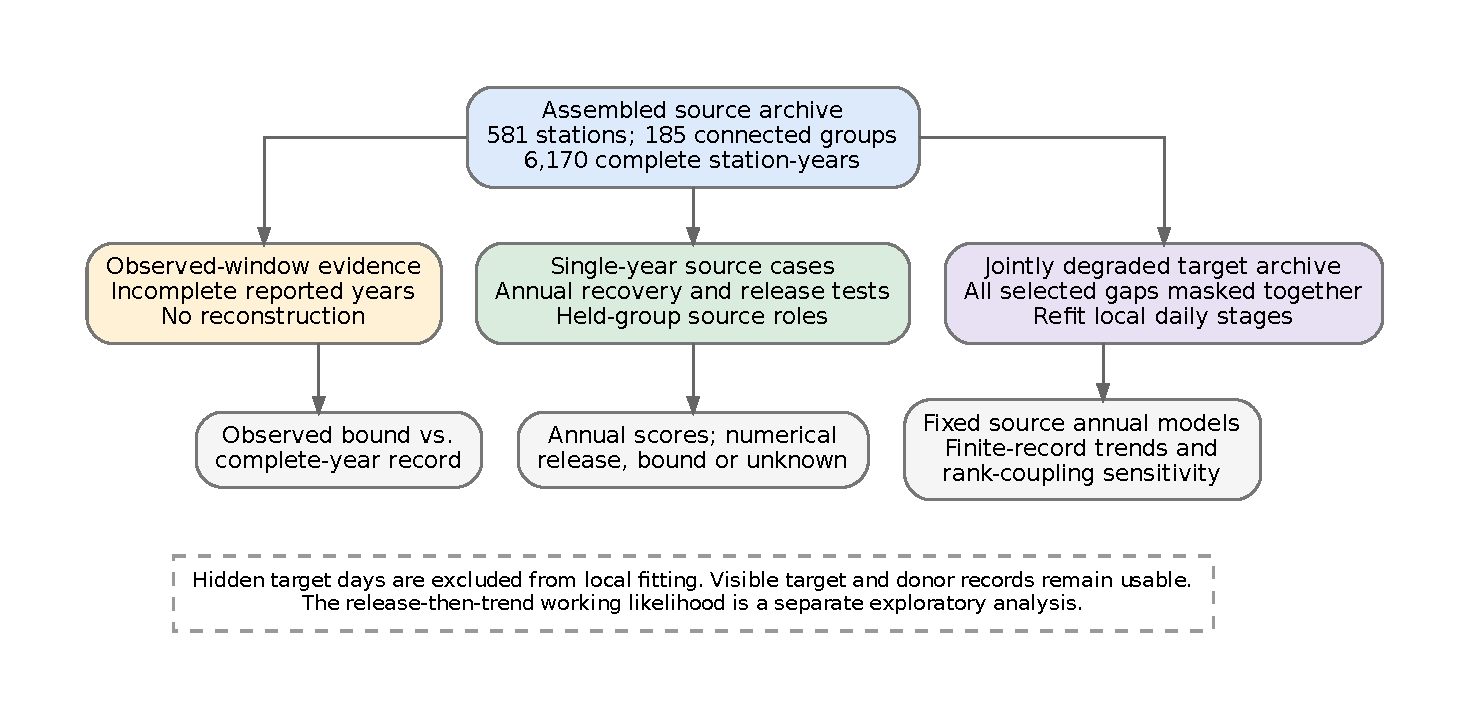
\includegraphics[width=\linewidth]{../wrr_tr/figures/architecture/fig1_evidence_actual.pdf}
\caption{Evidence layers in the leakage-safe benchmark. Observation-only witnesses test whether an incomplete year contains a fully observed 30-day window above the complete-year record; single-year source cases evaluate annual recovery and release; jointly degraded archives mask every selected target year before any local fit and score finite-record trends. Hidden target days never enter the local fit. Takeaway: separating observation-only, annual and whole-archive evidence keeps evaluation quantities out of fitting and selection.}
\label{fig:architecture}
\end{figure}

\begin{figure}[t]
\centering
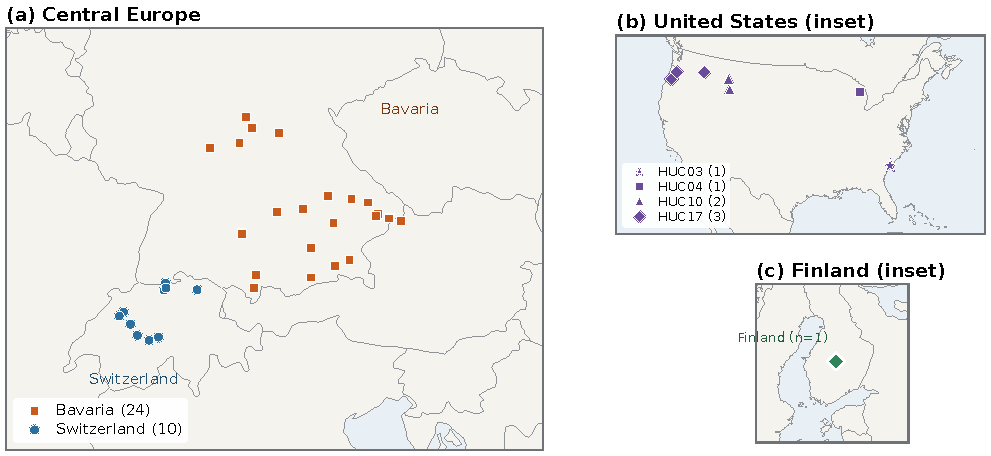
\includegraphics[width=\linewidth]{figures/study_stations.pdf}
\caption{Study-station locator map. The forward cohort contains 24 Bavarian and 10 Swiss stations in Central Europe (a), seven USGS stations in four HUC regions (b), and one Finnish reference site (c) that is not used in forward scoring. Country outlines are Natural Earth 1:50m; this is a locator map, not a basis for area, elevation or discharge covariates. Takeaway: the long-complete cohort is concentrated in Bavaria and Switzerland and is a monitoring-network sample, not a random river sample.}
\label{fig:sample}
\end{figure}

\begin{figure}[t]
\centering
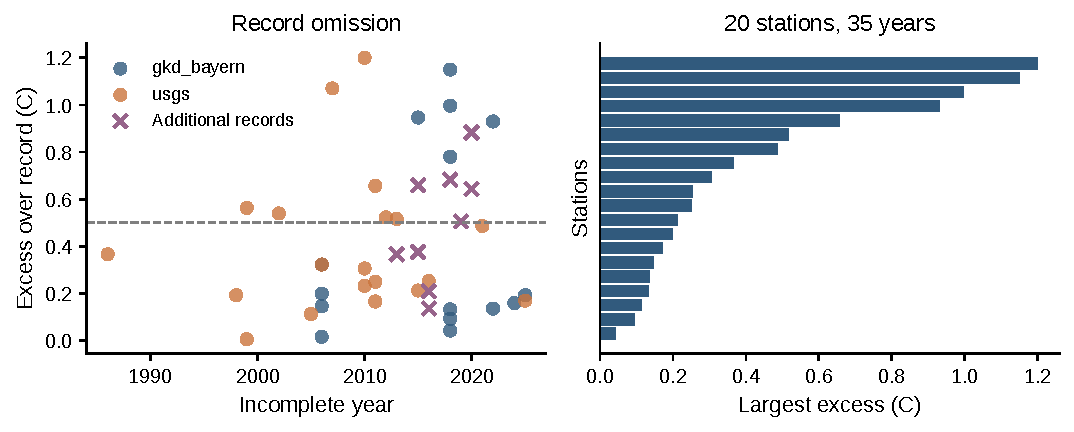
\includegraphics[width=\linewidth]{../wrr_tr/figures/simple_research/01_observed_records.pdf}
\caption{Observed heat evidence discarded by completeness screening. Left: largest fully observed 30-day window above the complete-year H30 record for each incomplete year; right: per-station maximum excess. Crosses are additional approved-record witnesses with sparse complete support and are not in the long-record denominator. Takeaway: 35 incomplete station-years at 20 stations contain observed windows above every complete-year H30, so a completeness screen is not evidence that heat information is absent.}
\label{fig:observed}
\end{figure}

\begin{figure}[t]
\centering
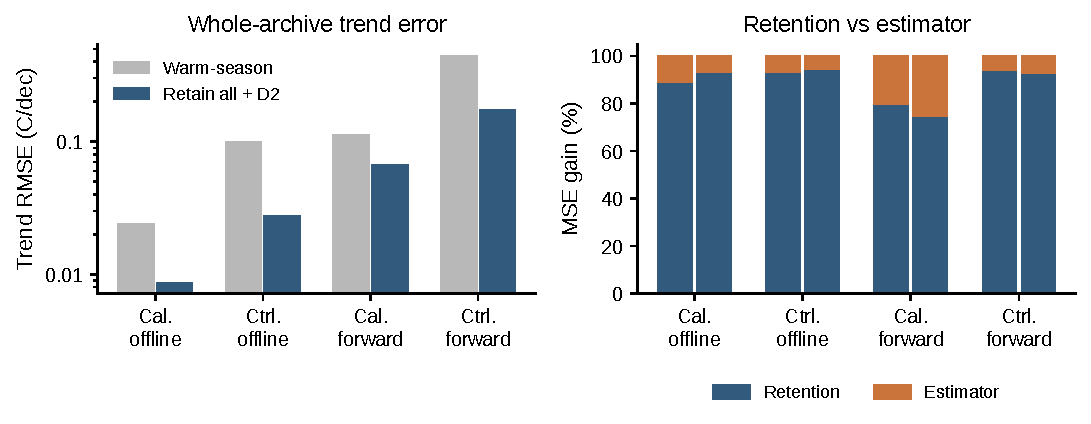
\includegraphics[width=\linewidth]{../wrr_tr/figures/simple_research/03_archive_factorial.pdf}
\caption{Whole-archive trend error and the retention/estimator decomposition. Left: trend RMSE on common station-repetition rows for warm-season screening and all-year recovery under D2, with archive and station/group counts. Right: percentage MSE gain from retention and estimator changes; paired bars use each method's own four-cell count. Takeaway: all-year recovery lowers the absolute slope error in 630 of 805 controlled-gap archives, raises it in 169 and leaves 6 numerically unchanged, so the aggregate gain is not universal.}
\label{fig:trend}
\end{figure}

\begin{figure}[t]
\centering
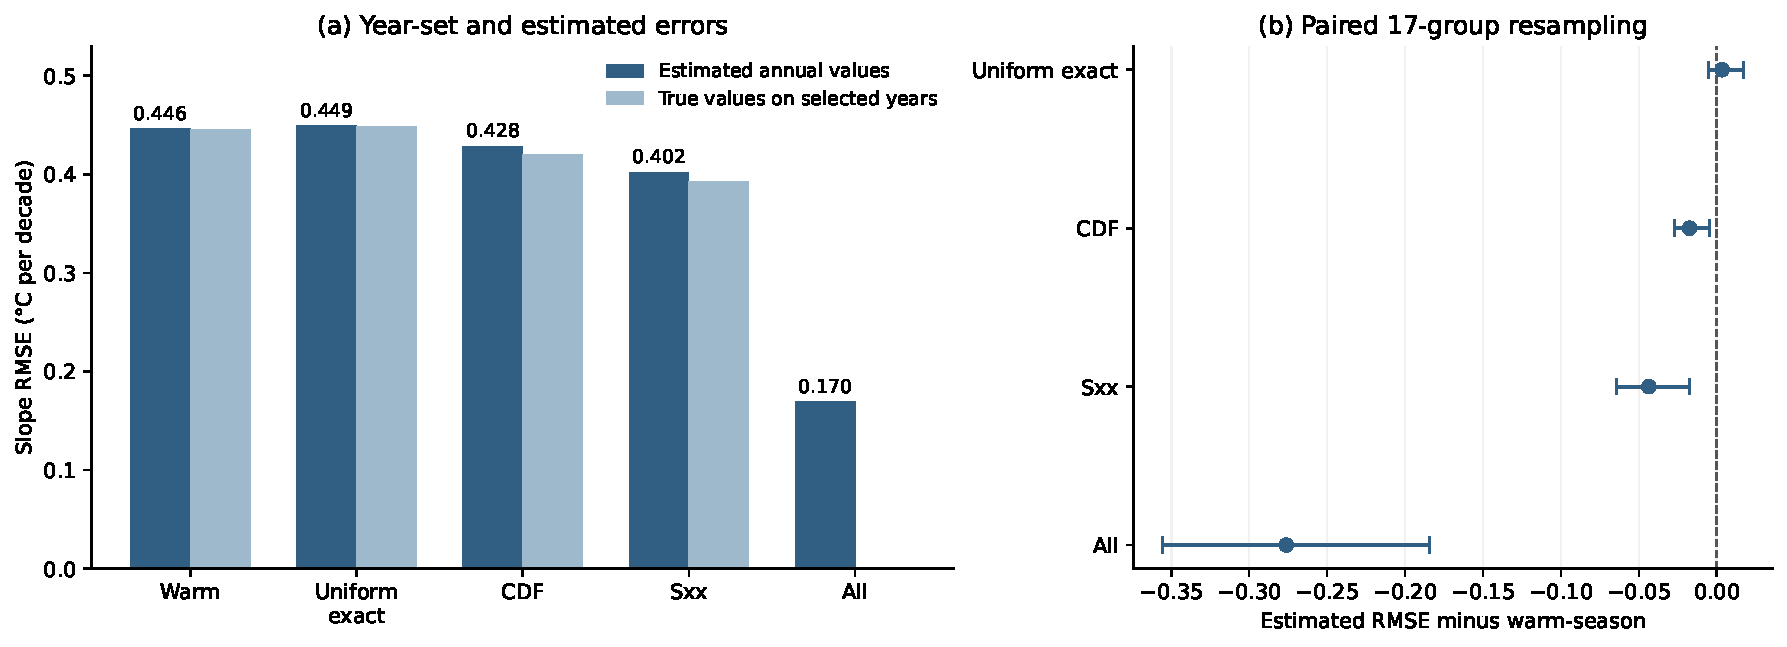
\includegraphics[width=\linewidth]{../wrr_tr/figures/process_revision/03_time_support.pdf}
\caption{Fixed-count year selection on 805 controlled-gap archives. Left: slope RMSE for warm-season screening, uniform exact subset averaging, CDF and $S_{xx}$ selection, using estimated annual values and complete-year H30 on the same selected years; all-year recovery is the reference. Right: comparator-minus-warm-season RMSE differences with paired 95\% percentile intervals from 10{,}000 resamples of 17 connected groups. Takeaway: CDF and $S_{xx}$ improve on warm-season screening at a fixed count, but all-year recovery remains closer to the complete-record slope (0.170 versus 0.428 and 0.402\,$^{\circ}$C/10a).}
\label{fig:selection}
\end{figure}

\begin{figure}[t]
\centering
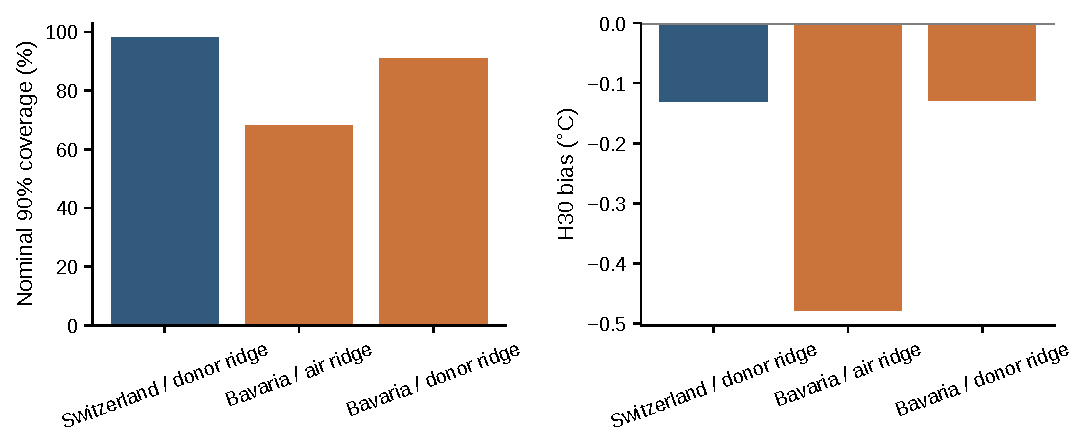
\includegraphics[width=\linewidth]{../wrr_tr/figures/process_revision/02_region_recovery.pdf}
\caption{Hidden-peak recovery by region and daily reconstructor. Left: nominal 90\% interval coverage; right: median bias (recovered minus complete-year H30). Bavarian air-ridge intervals cover 67.9\% of hidden peaks with a $-0.479$\,$^{\circ}$C bias, versus 90.8\% (Bavaria) and 98.1\% (Switzerland) for donor ridges; cases are not matched across reconstructors. Takeaway: recovery fails where local water information is absent, not merely where the calendar rule is imperfect.}
\label{fig:failure}
\end{figure}

\begin{figure}[t]
\centering
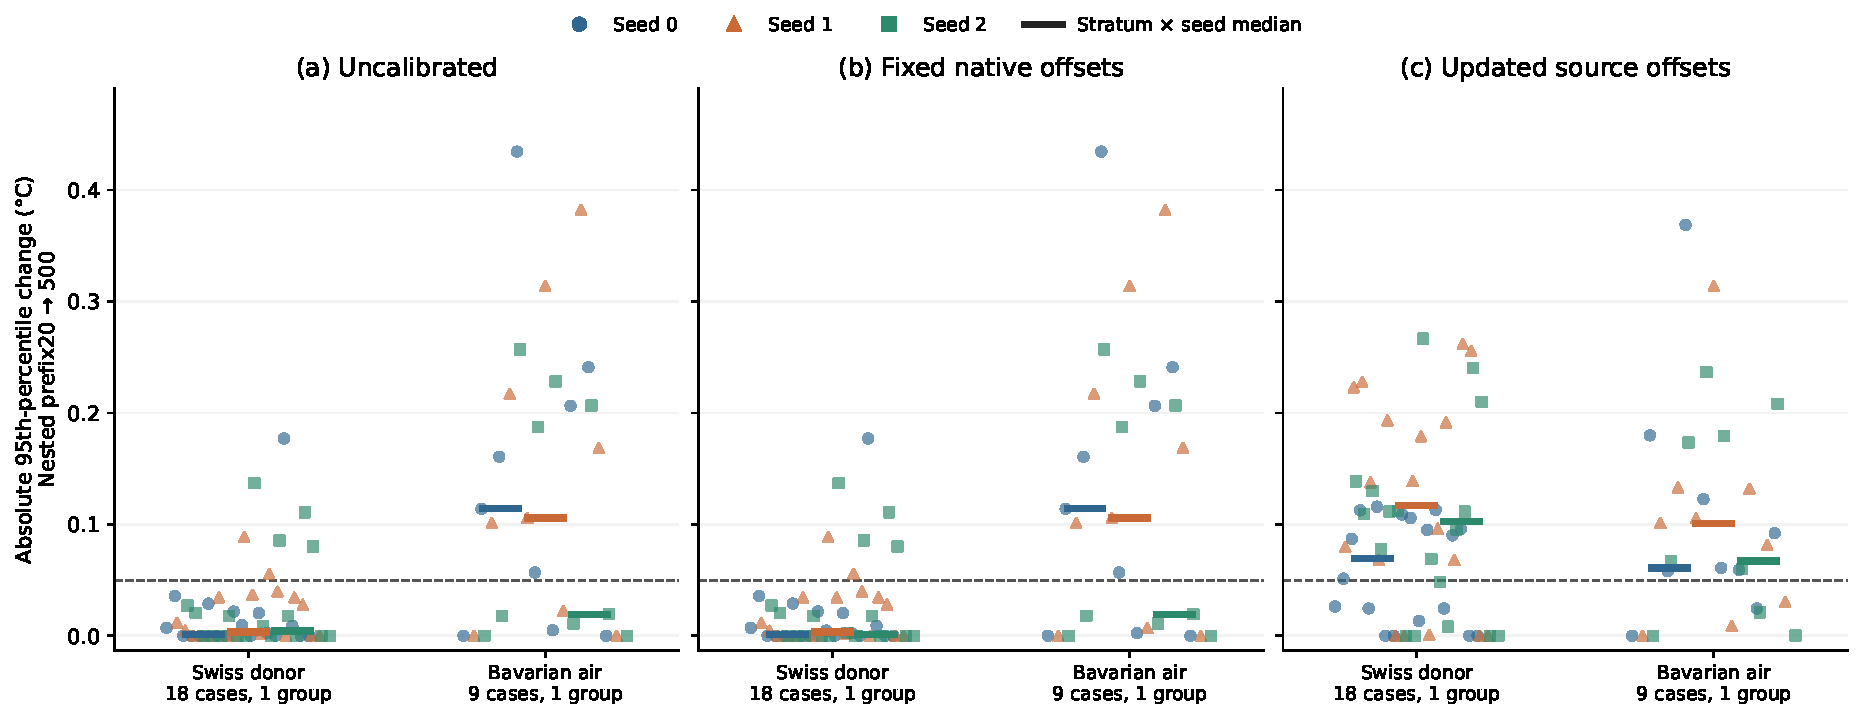
\includegraphics[width=\linewidth]{../wrr_tr/figures/process_revision/04_trajectory_budget.pdf}
\caption{Numerical sensitivity to the residual-bridge budget. Absolute change in the 95th-percentile endpoint between nested 20- and 500-path runs for the same 27 target cases under uncalibrated, fixed-offset and re-estimated-offset settings; colors are seeds and horizontal marks are stratum medians. The 0.05\,$^{\circ}$C line is a numerical diagnostic. Takeaway: the 20-path budget is a numerical-error floor; 500 paths on two target groups establish neither convergence nor a preferred estimator.}
\label{fig:budget}
\end{figure}
}{}

\section{Results}

\subsection{Observed windows in incomplete years remain facts}

\textbf{Incomplete years can contain observed 30-day windows that exceed every complete-year $\mathrm{H30}$ at the same station.} At 20 of 96 eligible stations, 35 incomplete station-years contain a fully observed 30-day window above the maximum complete-year $\mathrm{H30}$ (Figure~\ref{fig:observed}); six stations exceed the complete-year record by more than 0.5\,$^{\circ}$C. Of the 35 witnesses, 32 pass the 90\% warm-season rule and 31 pass the 95\% annual-coverage rule. Strict complete-year selection discards all 35; the warm-season rule admits 19 incomplete years whose windows exceed the accepted record of the other accepted years. Only two warm-season-excluded witnesses exceed the largest accepted window, by 0.150 and 0.113\,$^{\circ}$C. At an assumed 0.05\,$^{\circ}$C window error both increments exceed twice that error; at 0.10\,$^{\circ}$C neither does. The comparison is retrospective, after setting the evaluated year aside, not a sequence of records announced in historical time. Another incomplete year could still be warmer, and measurement error or a changed sensor location can affect physical interpretation. We treat this as a data-use principle: preserve observed windows as lower bounds, and do not equate a completeness screen with the absence of heat information. It is not a separate main contribution.

\subsection{Screening versus reconstruction at the trend scale}

\textbf{Against the trend's own sampling error, severe 30--90-day controlled gaps make screening costly and reconstruction effective, while realistic gap calendars leave both differences below trend uncertainty.} Table~\ref{tab:trend_signal_stations} and Table~\ref{tab:trend_signal_cohorts} report the complete-record signal and the archive-level errors. The complete-record reference is itself weakly constrained: across 41 stations and a median of 14 reference years, the median OLS $\mathrm{H30}$ slope is 0.754\,$^{\circ}$C/10a, its median classical SE is 0.590\,$^{\circ}$C/10a, and the median interannual $\mathrm{H30}$ SD is 1.011\,$^{\circ}$C; only 3 stations have OLS $p<0.05$ and 4 have tie-corrected Mann--Kendall $p<0.05$. Those Mann--Kendall values include a tie correction but no autocorrelation correction; modified variance and trend-free prewhitening tests \citep{hamed1998,yue2002} are the appropriate inference when serial dependence can be estimated, and we do not treat the reported values as autocorrelation-robust. The median absolute difference between OLS and Sen slopes is 0.102\,$^{\circ}$C/10a, so the choice of slope estimator is not negligible. This weak signal is why we scale errors by the slope SE rather than by the slope itself: the 0.446\,$^{\circ}$C/10a screening error is large against a 0.590\,$^{\circ}$C/10a SE but modest against a 0.754\,$^{\circ}$C/10a slope.

Annual recovery is similar for D2 and the stochastic comparator (median MAE 0.337 vs 0.336\,$^{\circ}$C; 90\% coverage 89.3\% vs 89.8\%) and both improve on the daily plug-in (0.428\,$^{\circ}$C), so the trend contrast is not a simple consequence of annual-point accuracy. The two estimators trade availability against precision. On common archives the stochastic comparator has the lower trend RMSE (0.147 vs 0.164\,$^{\circ}$C/10a controlled, $n{=}738$; 0.051 vs 0.062 calendar, $n{=}701$), but it produces no estimate on 82 of 820 controlled and 119 of 820 calendar archives, where D2 still yields values with RMSE 0.244 and 0.093\,$^{\circ}$C/10a. D2 is therefore the availability-complete option rather than the accuracy winner; we state this trade-off in the decision table instead of claiming a uniform advantage.

Under empirical gap calendars, warm-season screening and all-year reconstruction give RMSEs of 0.114 and 0.067\,$^{\circ}$C/10a, both well below the median SE. The median $|e|/$SE is 0.002 (P90 0.279) for screening and 0.000 (P90 0.095) for reconstruction, with 3 versus 0 sign flips. Under controlled 30--90-day gaps, reconstruction reduces RMSE from 0.446 to 0.170\,$^{\circ}$C/10a, the share of archives exceeding one SE from 13.42\% to 0.75\%, and sign flips from 53 to 16. The 0.446\,$^{\circ}$C/10a screening RMSE is 59.1\% of the median reference slope, but this is an aggregate error-to-slope ratio, not a per-archive relative underestimate: the median per-archive $|e|/$SE is 0.357 and 13.42\% of archives exceed one SE.

The cohort improvement is not universal at the archive level. All-year recovery has a smaller absolute slope error in 630 of 805 controlled-gap archives, a larger error in 169, and a numerically unchanged error in 6; in the empirical calendars the counts are 231, 57 and 530. Among the 288 calendar archives whose selected year set changes, 231 improve and 57 worsen. Numerical equality is an arithmetic $10^{-12}$\,$^{\circ}$C/10a tolerance, not practical equivalence. These counts describe station/mask combinations in the same opened archive rather than independent rivers, and a lower cohort RMSE does not imply that every archive should be recovered and released. Figure~\ref{fig:trend} summarizes the archive-level trend errors and the year-set/reconstruction decomposition.

\begin{table}[t]
\centering
\small
\caption{Complete-record H30 trend signal at the 41 forward stations. Slopes and standard errors use each station's saved reference-year set. SE denotes the classical OLS slope standard error and excludes autocorrelation.}
\label{tab:trend_signal_stations}
\begin{tabular}{lr}
\hline
Statistic & Value \\
\hline
Stations & 41 \\
Median reference years & 14 \\
Median OLS H30 slope ($^{\circ}$C/10a) & 0.754 \\
Median OLS slope SE ($^{\circ}$C/10a) & 0.590 \\
Stations with OLS $p<0.05$ & 3 \\
Stations with Mann--Kendall $p<0.05$ & 4 \\
Median $|\mathrm{OLS}-\mathrm{Sen}|$ slope ($^{\circ}$C/10a) & 0.102 \\
Median H30 interannual SD ($^{\circ}$C) & 1.011 \\
\hline
\end{tabular}
\end{table}

\begin{table*}[t]
\centering
\small
\caption{Archive-level H30 slope error scaled by the station's classical OLS slope standard error. Controlled: 30--90-day gaps; Calendar: empirical gap calendars. RMSE is in $^{\circ}$C/10a. $e$ is the estimated minus the complete-record slope.}
\label{tab:trend_signal_cohorts}
\resizebox{\linewidth}{!}{%
\begin{tabular}{llrrrrrrrr}
\hline
Family & Scheme & $n$ & RMSE & Median & P90 & $>1$ SE & Sign & Infl. & Weak \\
 & & & & $|e|/$SE & $|e|/$SE & (\%) & flips & (\%) & flips \\
\hline
Controlled & Warm-season 90\% & 805 & 0.446 & 0.357 & 1.148 & 13.42 & 53 & 21.49 & 43 \\
Controlled & CDF & 805 & 0.428 & 0.346 & 1.120 & 12.55 & 51 & 20.27 & 42 \\
Controlled & $S_{xx}$ & 805 & 0.402 & 0.315 & 0.997 & 9.94 & 42 & 17.93 & 35 \\
Controlled & All years & 805 & 0.170 & 0.108 & 0.458 & 0.75 & 16 & 3.66 & 16 \\
\hline
Calendar & Warm-season 90\% & 818 & 0.114 & 0.002 & 0.279 & 0.24 & 3 & 1.78 & 3 \\
Calendar & CDF & 818 & 0.098 & 0.002 & 0.195 & 0.00 & 5 & 1.13 & 5 \\
Calendar & $S_{xx}$ & 818 & 0.086 & 0.002 & 0.174 & 0.12 & 4 & 0.94 & 4 \\
Calendar & All years & 818 & 0.067 & 0.000 & 0.095 & 0.12 & 0 & 0.55 & 0 \\
\hline
\end{tabular}}
\par\smallskip\footnotesize The year-set-only uniform-exact control (not shown) has RMSE 0.449 (controlled) and 0.135 (calendar) $^{\circ}$C/10a and 55/8 sign flips; its archive-level estimates are not saved, so error/SE ratios are undefined. Calendar medians are diluted by identical year sets: restricted to the 288 calendars whose warm-season and all-year sets differ, screening gives RMSE 0.191 with median and P90 $|e|/$SE of 0.151 and 0.559, against 0.112, 0.026 and 0.225 for all-year recovery. All 200 FOEN (Swiss) calendars have zero screening error because their real gaps are too short to change the retained set. Infl. is the total-uncertainty inflation $\sqrt{1+\mathrm{mean}((e/\mathrm{SE})^2)}-1$; Weak flips are the sign flips at stations with $|\beta|<1$ SE, where the complete-record sign is itself uncertain.
\end{table*}

\noindent\textbf{Interpretation.} The complete-record reference slope is itself weakly constrained: across 41 stations and a median of 14 reference years, the median OLS H30 slope is 0.754 $^{\circ}$C/10a, its median classical SE is 0.590 $^{\circ}$C/10a, and the median interannual H30 SD is 1.011 $^{\circ}$C; only 3 stations have OLS $p<0.05$ and 4 have tie-corrected Mann--Kendall $p<0.05$. Under empirical gap calendars, warm-season screening and all-year reconstruction give RMSEs of 0.114 and 0.067 $^{\circ}$C/10a, both well below the median SE (0.590 $^{\circ}$C/10a); the median $|e|/$SE is 0.002 (P90 0.279) for screening and 0.000 (P90 0.095) for reconstruction, with 3 versus 0 sign flips. Under controlled 30--90-day gaps, reconstruction reduces RMSE from 0.446 to 0.170 $^{\circ}$C/10a, the share of archives exceeding one SE from 13.42\% to 0.75\%, and sign flips from 53 to 16. The 0.446 $^{\circ}$C/10a screening RMSE is 59.1\% of the median reference slope (0.754 $^{\circ}$C/10a), but this is an aggregate error-to-slope ratio, not a per-archive relative underestimate: the median per-archive $|e|/$SE is 0.357 and 13.42\% of archives exceed one SE. Because the OLS SE excludes autocorrelation, the error/SE ratios are lower bounds on the trend's sampling uncertainty. Expressed as inflation of total trend uncertainty, warm-season screening adds 21.49\% under controlled gaps and 1.78\% under empirical calendars, while all-year recovery adds 3.66\% and 0.55\%. 43 of the 53 controlled-gap screening flips and 16 of the 16 recovery flips occur at stations with $|\beta|<1$ SE, and no flip occurs at any of the three stations with $|t|\ge 2$.


\subsection{Fixed-count year selection helps but does not replace recovery}

\textbf{Calendar-aware year selection recovers part of the lost time support at a fixed count, but all-year reconstruction remains closer to the complete-record slope.} On the 805 controlled-gap archives, the warm-season rule retains 9.59 years on average and gives RMSE 0.446; CDF gives 0.428 and $S_{xx}$ 0.402, while all-year recovery gives 0.170. Paired group-resampling intervals for CDF-minus-warm and $S_{xx}$-minus-warm are $[-0.027,-0.005]$ and $[-0.065,-0.017]$; the all-year-minus-warm interval is $[-0.356,-0.184]$. Both calendar controls change 367 and 376 warm-season selections, respectively, and the direction persists with station- or group-equal weights and after each of the 17 group deletions. The CDF and $S_{xx}$ controls also reduce the year-set-only RMSE from 0.446 to 0.420 and 0.393, so part of their gain comes from placing years rather than from reconstruction. On the 468 archives that offer a nontrivial same-count choice, warm, CDF and $S_{xx}$ RMSEs are 0.394, 0.359 and 0.303; all-year recovery remains at 0.170 on the full cohort. The year-set-only error under warm-season screening is 0.446 and the reconstruction error on that set is 0.002; the near-zero reconstruction term is why all-year recovery is closer, not because the year set is irrelevant.

On the 818 empirical calendars, warm-season RMSE is 0.114, CDF 0.098, $S_{xx}$ 0.086, and all-year 0.067. The CDF-minus-warm paired interval $[-0.045,0.0004]$ includes zero; the $S_{xx}$ and all-year intervals are below zero. Only 280 of 818 calendars offer a nontrivial same-count choice, and 530 already retain every incomplete year, so the calendar-cohort ranking cannot be transported to the controlled-gap cohort. The value of year placement depends on the gap family and on which selection margin is available.

Station and group summaries show the same asymmetry. All-year recovery improves on warm-season screening at every station (41/41) and group (17/17) in the saved 805-archive summaries. CDF is worse than warm-season screening at 14 of 41 stations and 3 of 17 groups; $S_{xx}$ is worse at 7 of 41 and 2 of 17. The aggregate improvement does not imply that every station or group benefits from a same-count rule. Figure~\ref{fig:selection} shows the fixed-count comparison and the paired differences.

\subsection{Failure conditions concentrate where local water information is absent}

\textbf{Failures concentrate where recovery lacks local water information, not where the calendar rule is merely imperfect.} Hidden-peak fractions are similar in Bavaria (58.4\%) and Switzerland (56.6\%), but reconstruction support differs (Figure~\ref{fig:failure}). Bavarian air-ridge 90\% intervals cover 67.9\% of hidden peaks with a median bias of $-0.479$\,$^{\circ}$C; 30.2\% of references exceed the upper endpoint. Donor-ridge coverage is 90.8\% in Bavaria and 98.1\% in Switzerland, with biases $-0.129$ and $-0.130$\,$^{\circ}$C. Daily out-of-fold residual scales are 1.054\,$^{\circ}$C for the Bavarian air ridge, 0.673\,$^{\circ}$C for the Bavarian donor ridge, and 0.455\,$^{\circ}$C for the Swiss donor ridge. These are conditional associations among different cases, not a controlled change of reconstructor at the same station.

Common geometric support alone has a regional cell-frequency total variation of 0.228. Identical min-count weights reduce that distance to zero and yield coverage 98.72\% in Switzerland versus 82.68\% in Bavaria, a 16.04-point gap; equal-cell weighting gives 17.62 points. Adding reconstructor class retains only 289 of 1,983 Bavarian cases and 472 of 1,119 Swiss cases; the standardized coverage gap is 3.69 points, but Switzerland supplies no air-ridge counterpart to the main Bavarian failure layer. Removing 85.4\% of Bavarian cases cannot estimate how much reconstructor choice explains the original regional gap, and training complete-year counts remain imbalanced after weighting (absolute standardized differences above 2.7). Deleting one connected group leaves the geometric contrast positive (12.39--17.77 points), but the reconstructor-conditioned contrast can reverse sign (minimum $-1.12$ points). The cause of the regional difference remains unidentified; support loss, history imbalance, provider and river type are entangled, and we do not claim a causal mechanism.

Two bounded diagnostics follow: an open-source candidate-provider sensitivity and a zero-flow proxy analysis. Neither supplies a validated correction.

\IfFileExists{open_source_flow.tex}{\subsection{Open-source model sensitivity}
A practical question for reuse is whether the comparison survives replacement of the restricted source providers by openly available products. As a candidate route, we refitted the source models on seven candidate providers with recorded reuse paths while retaining the target masks, daily features and plug-in baselines. On the crossed/forward cohort, the D2 trend RMSE changes from 0.164 to 0.158 $^{\circ}$C per decade and the classical RMSE from 0.147 to 0.156, over 738 four-way common pairs in 17 groups. The D2 retention fraction in the symmetric MSE decomposition falls from 93.9\% to 93.7\% on 807 factor cases, and nominal 95\% D2 interval coverage from 88.0\% to 87.6\% on 820 coverage cases. The substantive conclusions are unchanged. This is a candidate open reproducibility route, not a legal clearance: LUBW rights and the provenance of neighbour records still require confirmation. The candidate-source tables are descriptive, repetitions are not independent climates, and the filtered inputs remain processed study data rather than provider-native records. Global water-temperature modelling \citep{vanvliet2011} and recent assessments of water-temperature data coverage \citep{diaz2025} make such a route plausible, but its legal and operational status is not established here.

\subsection{Flow proxy diagnostic}
Flow can modify river thermal response \citep{vanvliet2011}, process models use discharge explicitly \citep{toffolon2015}, and regulated or groundwater-influenced reaches can change interval performance \citep{diaz2025}. Our evidence is diagnostic and associational. In the 336-station, 6,479-station-year USGS missingness sample, 21 stations in 17 groups recorded at least one zero-flow day and 16 stations in 14 groups recorded at least 30. A station-fixed conditional logit related a warm-season-incomplete year (the hidden-peak condition) to within-station standardized summer air temperature, within-station standardized summer log flow and a linear trend (per decade). In the flow-adjusted model, the odds ratio for the flow term is 0.594 [0.409, 0.813] for the recorded-zero cohort (282 station-years, 129 events) and 0.474 [0.265, 0.676] for the at-least-30-zero-day cohort (215 station-years, 104 events). Air temperature is 0.993 [0.659, 1.305] and 0.855 [0.580, 1.275]; the trend term is 1.198 [0.520, 1.883] and 1.292 [0.597, 2.132]. In the large fewer-than-30-zero-day cohort the flow odds ratio is 0.969 [0.897, 1.046]. The lower hidden-peak odds is an association in this proxy cohort, not evidence that low flow protects against underestimation. Zero flow is a historical proxy: no recorded zero does not prove perennial flow, and a zero does not identify an intermittent river, sensor exposure or a dry bed. The flow-adjusted subsets are smaller, so differences from the air-only model are not a mediation estimate.

The opened flow-comparator experiment provides a separate, non-causal check. It contains 255 sites, 8,999 complete climatic years and 134,925 cases; paired comparisons cover 210 sites, while the full 255-site cohort spans 17 HUC2 region groups. Historical D2 and single-donor Ridge baselines are already available. Donor-dependent methods are available on 81.7\% of crossed/all eligible cases versus 100\% for historical D2, and they do not lower paired mean absolute error (MAE; Table~\ref{tab:ems_flow_comparators}). In the danger scope, MOVE.1 has MAE 0.1062, the stochastic bridge 0.1038, single-donor Ridge 0.0896 and historical D2 0.0745. The flow comparators therefore show no accuracy gain here, and their lower availability is material.

\begin{table}[t]
\centering\footnotesize
\caption{Paired log-flow MAE in the opened flow-comparator cohort, crossed/all scope (66,099 common cases, 210 sites; the 255-site cohort spans 17 HUC2 region groups). ``Not worse'' is the percentage of sites where the left estimator's MAE does not exceed the right estimator's.}
\label{tab:ems_flow_comparators}
\resizebox{\linewidth}{!}{%
\begin{tabular}{lrrr}
\toprule
Comparison & Left MAE & Right MAE & Not worse (\%)\\
\midrule
MOVE.1 vs single-donor Ridge & 0.0734 & 0.0602 & 15.2\\
MOVE.1 vs historical D2 & 0.0734 & 0.0495 & 13.3\\
Stochastic bridge vs historical D2 & 0.0716 & 0.0495 & 28.1\\
\bottomrule
\end{tabular}}
\end{table}

The limitations are explicit: the zero-flow class is a station-level proxy; no 34-station FOEN/GKD daily flow merge was performed; air2stream-8 was not retrained with flow; no causal mechanism is identified; and rights and coverage for the required flow data remain unresolved. The comparator experiment is one opened positive-flow perennial subset, not a new blind transfer or a 20-seed stability claim.
}{}

In all cases the proxy is an association, not a flow correction. The Bavarian air-ridge failure remains an information-condition result, not a causal low-flow attribution.

A seven-day (H7) refit in the research repository changed the estimator-level comparison: the median paired MAE reduction relative to the stochastic comparator was 2.94\% in the crossed family and 4.85\% in the calendar family, CRPS and tail CRPS improved in 20/20 seeds, and trend-interval coverage for the missingness component remained near 81\%. Because H7 is a different target, it is a robustness check in Supporting Information Table~S5, not confirmation of the $\mathrm{H30}$ results.

\section{Discussion}

\subsection{A practical decision table}

The results support a simple decision rule: reconstruct when the gap is severe and the archive supplies local water information; preserve observed windows when only a threshold exceedance is needed; and state the reference-year set and selection rule whenever a slope is reported. Table~\ref{tab:decision} makes the rule operational and attaches the expected error in slope-SE units. The table is a decision aid, not a guarantee: the error summaries are descriptive quantiles from the evaluated archives, not probabilities for a new river. History length and neighbor availability enter the table qualitatively because the case study does not support a validated threshold: mean visible donors are 7.3 in Switzerland and 5.5 in Bavaria, and the minimum reference set is 7 years. These are context for the evaluated cohort, not universal decision cutoffs.

\begin{table}[p]
\centering
\scriptsize
\caption{Practical decision table for incomplete annual $\mathrm{H30}$ records. Error columns give the median and 90th percentile of $|e|/$SE, where $e$ is the estimated minus the complete-record slope and SE is the station's classical OLS slope standard error. These are descriptive summaries of the evaluated archives, not guarantees for a new station.}
\label{tab:decision}
\resizebox{\linewidth}{!}{%
\begin{tabular}{@{}>{\raggedright\arraybackslash}p{0.25\textwidth}>{\raggedright\arraybackslash}p{0.21\textwidth}>{\raggedright\arraybackslash}p{0.30\textwidth}>{\raggedright\arraybackslash}p{0.20\textwidth}@{}}
\toprule
Situation & Recommended output & Expected slope error & Evidence \\
\midrule
Any gap; only a threshold exceedance is needed; a fully observed 30-day window exists. & Report $L_y$ as an observed lower bound; do not label it an annual $\mathrm{H30}$. & Bound is exact for the window; not an annual slope estimator. Adds only 2 of 35 witnesses beyond the warm-season rule, by 0.150 and 0.113\,$^{\circ}$C. & 2,700 station-years at 96 stations. \\
Typical calendar (median longest run 4 days; 88\% shorter than 30 days); $\ge$10 reference years; local or donor history. & Reconstruct all supported years within $Y_i$. & Median 0.000, P90 0.095 SE; 0 of 818 sign flips. & 818 empirical calendars. \\
Severe 30--90-day summer gap overlapping the climatological peak; $\ge$7 reference years; donor or local history. & Reconstruct all supported years within $Y_i$. & Median 0.108, P90 0.458 SE; 0.75\% above 1 SE; 16 of 805 sign flips. & 805 controlled gaps. \\
Severe gap, but reconstruction is unavailable or no donor group exists. & Discard incomplete years; report the reduced-support slope and state $Y_i$. & Median 0.357, P90 1.148 SE; 13.42\% above 1 SE; 53 of 805 sign flips. & Same cohort. \\
A fixed year count is required (for example, a balanced panel). & Use CDF or $S_{xx}$ calendar selection, always retaining complete years. & Controlled: 0.346/1.120 (CDF), 0.315/0.997 ($S_{xx}$) SE. Calendar: 0.002/0.195 (CDF), 0.002/0.174 ($S_{xx}$). All-year remains 0.108/0.458 and 0.000/0.095. & 805 controlled and 818 calendar archives. \\
No local water history and no donor; air-only ridge; regulated or lake-influenced reach; hidden peak possible. & Do not release a calibrated annual value; report a bound, a widened interval, or an unknown. & 90\% coverage 67.9\%; median bias $-0.479$\,$^{\circ}$C; 30.2\% of references above the upper endpoint. & Bavarian air-ridge cases. \\
Flow or zero-flow proxy records are available. & Use as a diagnostic or screening covariate; do not apply a flow correction. & No validated error reduction in SE units; association only. & Zero-flow proxy; no air2stream-8 retraining. \\
\bottomrule
\end{tabular}}
\end{table}


Three implications follow. First, severe controlled gaps are not a case for completeness screening. Under 30--90-day gaps, screening's median error is about one-third of a slope SE, its 90th percentile exceeds one SE, and it flips the slope sign in 53 of 805 archives; reconstruction reduces those numbers to 0.108, 0.458 and 16. The flips concentrate where the record is already ambiguous: 43 of the 53 screening flips and all 16 recovery flips occur at stations whose complete-record slope is less than one SE from zero, and none of the three stations with $|t|\ge 2$ flips under either handling. Inflation of total trend uncertainty, $\sqrt{1+\mathrm{mean}((e/\mathrm{SE})^2)}-1$, is 21.5\% for screening against 3.7\% for reconstruction. The practical difference is large relative to the trend signal, which is itself only 0.754\,$^{\circ}$C/10a with a median SE of 0.590. Second, typical observed gaps are a different regime. The observed archive's median longest run is 4 days, and the empirical-calendar RMSEs of 0.114 and 0.067 are both below the median SE; the difference between screening and reconstruction is smaller than the trend uncertainty. The aggregate is diluted by unaffected archives: all 200 Swiss (FOEN) calendars leave the retained year set unchanged, and restricted to the 288 calendars whose retained sets do change, screening gives an RMSE of 0.191\,$^{\circ}$C/10a (median $|e|/$SE 0.151, P90 0.559) against 0.112 (0.026, 0.225) for all-year recovery. In that regime, the choice of screening versus reconstruction is less important than stating what was done and preserving the observed facts. Third, fixed-count selection is a partial remedy. CDF and $S_{xx}$ improve on the warm-season rule in aggregate, but all-year recovery improves further, and the calendar CDF interval includes zero. A same-count rule is appropriate when a balanced panel is required, not as a substitute for using supported years.

In practice, the table is applied in three steps. First, compute $L_y$ for every incomplete year and mark the years with a fully observed 30-day window. Second, fix $Y_i$ and count the reference years. Third, classify the gap by season and length, and check whether a donor or local water history is available. The table then returns a default action and the corresponding error scale. The action is a starting point for an archive-level audit, not a substitute for inspecting the specific river and the specific gap.

The decision table also marks the failure boundary. An air-only reconstruction without local water history or a donor group can produce a central value that looks precise but misses the hidden peak: 90\% coverage of 67.9\%, median bias $-0.479$\,$^{\circ}$C, and 30.2\% of references above the upper endpoint. In that situation the honest output is an observed lower bound, a widened interval, or an explicit unknown, not a calibrated annual value. Flow availability would help diagnose this boundary, but the zero-flow proxy does not supply a correction, and we did not retrain a flow-aware model.

\subsection{Relation to conformal prediction, multiple imputation, and cluster inference}

D2's recalibration is a per-quantile empirical offset stratified by difficulty class, analogous to conformalized quantile regression \citep{romano2019} but without its finite-sample guarantee, because calibration rows are reused, replicated by weight and correlated within classes. The 67.9\% Bavarian coverage is the expected failure mode when calibration and target conditions are not exchangeable. Weighted conformal prediction for covariate shift \citep{tibshirani2019}, adaptive conformal inference for time drift \citep{gibbs2021}, and methods that target conditional coverage \citep{gibbs2023} are the natural extensions. Quantile rearrangement handles crossing \citep{chernozhukov2010}, and quantile regression forests offer a distributional alternative \citep{meinshausen2006}. The present design does not implement these extensions; it diagnoses why a marginal conformal guarantee is not enough.

The stochastic comparator is closer to multiple imputation than to a single point predictor: it generates annual marginal distributions and couples them by residual bridges or ranks, then computes the slope for each realization. This preserves the margins but is not a draw from a joint posterior over daily paths. Rubin's rules require draws from a joint imputation model and congeniality between the imputation and analysis models \citep{rubin1987,little2019,meng1994}; the multiple-imputation literature treats both as design requirements, not post-hoc checks \citep{vanbuuren2018}. Rank coupling satisfies neither condition in general. A joint daily model (state-space, AR, or a probabilistic imputation network such as CSDI) would be the principled route \citep{tashiro2021}. Modern imputation baselines are also missing: Kalman smoothing and imputeTS \citep{moritz2017}, missForest \citep{stekhoven2012}, BRITS \citep{cao2018}, and SAITS \citep{du2023} were not run on the same masks. Their absence limits the claim from ``better than the daily plug-in'' to ``a useful benchmark comparator,'' not ``the best available imputation.''

Cluster inference is the third limit. The forward cohort has 41 stations in 17 connected groups; the 805 and 818 archives are station $\times$ repetition $\times$ setting combinations, not independent rivers. Group bootstrap intervals can be too narrow with few clusters \citep{cameron2008}. Wild cluster bootstrap or a mixed-effects model with station and group random effects would be preferable for the main contrasts. The station-mask repetitions are pseudo-replication: they describe variability within the opened archive, not independent climates. The same cohort has been used for multiple exploratory analyses, so the intervals are post-hoc summaries rather than confirmatory coverage statements; adaptive reuse of a holdout erodes its nominal validity \citep{dwork2015}. A locked test on stations not used in development remains the strongest missing validation. The leakage contract follows the data-leakage taxonomy of \citet{kapoor2023}, and the failure boundary is documented in the spirit of a model card \citep{mitchell2019}.

\subsection{Limitations}

The cohort is the long-complete tail of the archive: median 31 complete years versus 8 among the remaining 539 stations, with 24 of 42 evaluation stations in Bavaria and 10 of 41 forward stations in Switzerland. It is not a random river sample, and the conclusions are conditional on it.

The forward design has 41 stations in 17 connected groups, with two Swiss groups. Repeated masks and multiple settings are pseudo-replication, not independent hydroclimates. The regional, same-count, budget, H7 and flow diagnostics were developed after inspecting the same opened archive; they are exploratory, not preregistered confirmation.

The target is a finite-record slope on $Y_i$, not a climate-process trend. The OLS standard error excludes autocorrelation and is a lower bound; the trend intervals are group-bootstrap percentile intervals and are not calibrated at 95\%. Annual and trend intervals are distinct, and neither is a guarantee for a new station.

Observed gaps are much shorter than the controlled stress: median longest run 4 days, 11.93\% at least 30 days. The controlled 30--90-day gaps are a stress test, not an outage-frequency estimate. In the empirical calendars, many archives retain the same year set under all-year recovery, so practical gains occur only where the selected set changes. The comparison does not measure every donor's availability or a common outage cause.

The source includes LUBW observations whose reuse and redistribution terms are unresolved. All 13 estimator roles and 6 interval-calibration roles include positive-weight LUBW cases; the LUBW station is omitted from the local evaluation cohort, and the full eligible population is not reconstructed. Reviewer access to restricted material requires editorial and legal confirmation.

We did not complete daily discharge for all stations, retrain air2stream-8, or run modern imputation baselines (Kalman/imputeTS, missForest, BRITS, SAITS) and a joint-model multiple imputation on the same masks. The flow proxy is a diagnostic, not a correction. Forcing sensitivity using E-OBS \citep{cornes2018} or ERA5-Land \citep{munoz2021}, history-length and neighbor ablation, and a locked new-station confirmation were not completed. The pipeline is also not expressed as an explicit workflow DAG \citep{molder2021}, so end-to-end provenance depends on documentation rather than executable capture. H7 is reported only as a robustness check in Supporting Information Table~S5.

Finally, the regional contrast is not causal. Support loss, history imbalance, provider, river type and regulation are entangled; the reconstructor-conditioned contrast can reverse sign when one group is removed. The air-ridge undercoverage is consistent with missing flow information but does not identify a mechanism.

\section{Conclusions}

Severe controlled gaps favor reconstruction. Under 30--90-day gaps, screening incomplete years gives a slope RMSE of 0.446\,$^{\circ}$C/10a, a median error of 0.357 slope SE, 13.42\% of archives exceeding one SE, and 53 sign flips in 805 archives; restoring all supported years reduces these to 0.170, 0.108, 0.75\% and 16. Typical gaps are a different regime: under empirical calendars, screening and reconstruction inflate total trend uncertainty by 1.8\% and 0.5\%, with 3 and 0 sign flips; even restricted to the 288 calendars whose retained year sets change, screening stays below one slope SE at the 90th percentile. In that regime the difference between the two handling choices is smaller than the trend uncertainty.

Calendar-aware selection helps at a fixed count but does not replace recovery. CDF and $S_{xx}$ give 0.428 and 0.402\,$^{\circ}$C/10a under severe gaps and 0.098 and 0.086 under empirical calendars; the calendar CDF interval includes zero, while all-year recovery gives 0.170 and 0.067. All-year recovery improves on warm-season screening at every evaluated station and group, but not in every archive: 630 of 805 controlled-gap archives improve, 169 worsen, and 6 are numerically unchanged.

Recovery fails where local water information is absent. Bavarian air-ridge hidden-peak intervals cover 67.9\% at nominal 90\%, with a median bias of $-0.479$\,$^{\circ}$C and 30.2\% of references above the upper endpoint; donor-ridge coverage is 90.8\% in Bavaria and 98.1\% in Switzerland. The regional difference is not causal: support loss, history imbalance, provider and river type remain entangled, and the flow proxy is diagnostic only.

The practical conclusion is to preserve observed 30-day windows as facts, state the reference-year set and the year-selection rule for any slope, and report year-set error, reconstruction error and numerical sampling separately. The open-source \texttt{gapbench} 1.2.0 package makes the leakage-safe primitives reusable beyond this case study: observed-window bounds, finite-record slopes, calendar-only year selection, slope-error decomposition, group-disjoint splits, and archive masking. The benchmark is the contribution; the case study supplies its quantitative boundaries.
%
}{%
  \section*{Manuscript body}
  \noindent\textit{[Manuscript body to be inserted from \texttt{body.tex}.]}
  \IfFileExists{figures.tex}{\begin{figure}[t]
\centering
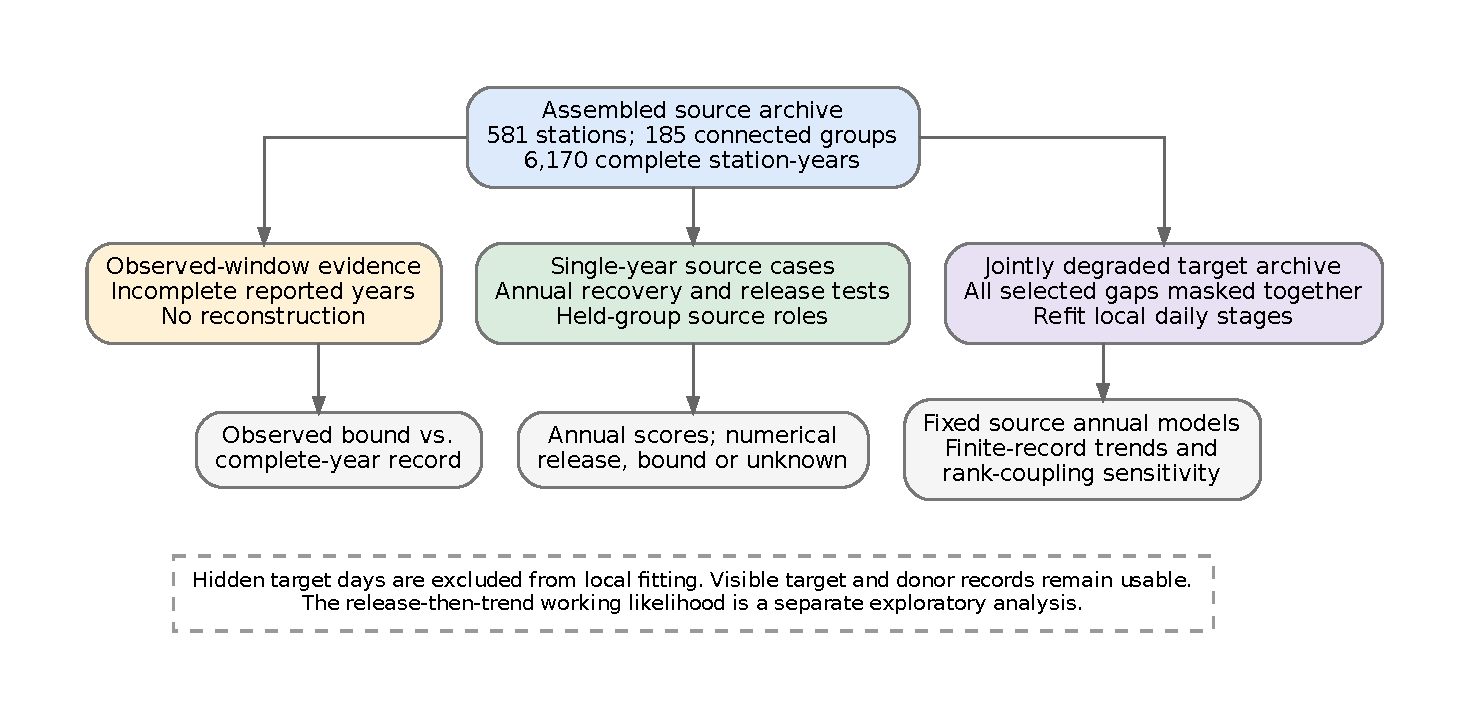
\includegraphics[width=\linewidth]{../wrr_tr/figures/architecture/fig1_evidence_actual.pdf}
\caption{Evidence layers in the leakage-safe benchmark. Observation-only witnesses test whether an incomplete year contains a fully observed 30-day window above the complete-year record; single-year source cases evaluate annual recovery and release; jointly degraded archives mask every selected target year before any local fit and score finite-record trends. Hidden target days never enter the local fit. Takeaway: separating observation-only, annual and whole-archive evidence keeps evaluation quantities out of fitting and selection.}
\label{fig:architecture}
\end{figure}

\begin{figure}[t]
\centering
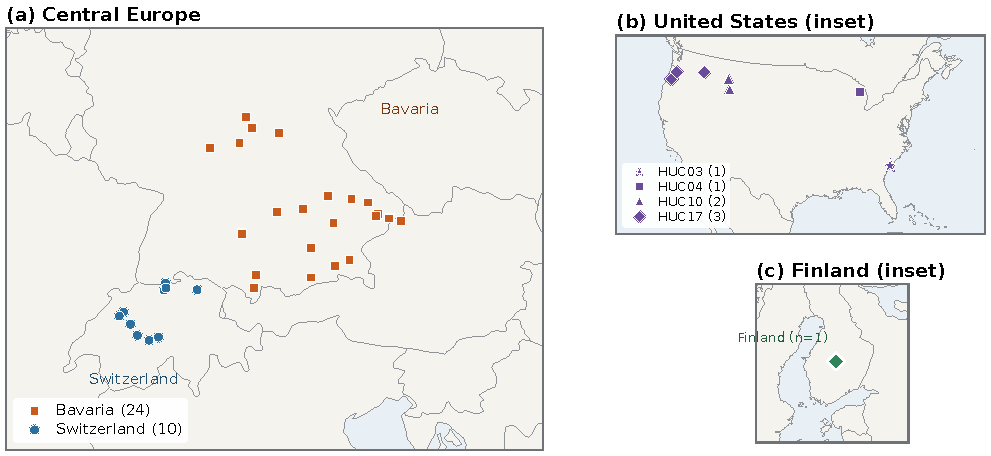
\includegraphics[width=\linewidth]{figures/study_stations.pdf}
\caption{Study-station locator map. The forward cohort contains 24 Bavarian and 10 Swiss stations in Central Europe (a), seven USGS stations in four HUC regions (b), and one Finnish reference site (c) that is not used in forward scoring. Country outlines are Natural Earth 1:50m; this is a locator map, not a basis for area, elevation or discharge covariates. Takeaway: the long-complete cohort is concentrated in Bavaria and Switzerland and is a monitoring-network sample, not a random river sample.}
\label{fig:sample}
\end{figure}

\begin{figure}[t]
\centering
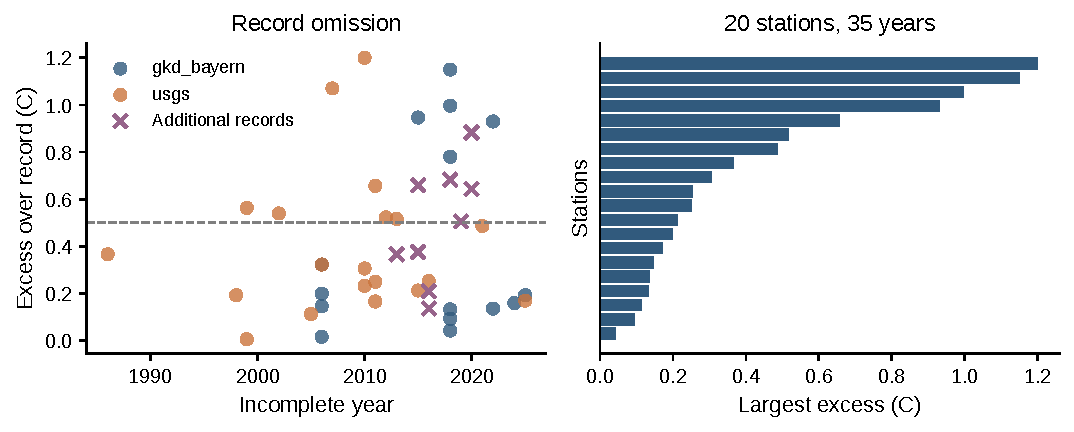
\includegraphics[width=\linewidth]{../wrr_tr/figures/simple_research/01_observed_records.pdf}
\caption{Observed heat evidence discarded by completeness screening. Left: largest fully observed 30-day window above the complete-year H30 record for each incomplete year; right: per-station maximum excess. Crosses are additional approved-record witnesses with sparse complete support and are not in the long-record denominator. Takeaway: 35 incomplete station-years at 20 stations contain observed windows above every complete-year H30, so a completeness screen is not evidence that heat information is absent.}
\label{fig:observed}
\end{figure}

\begin{figure}[t]
\centering
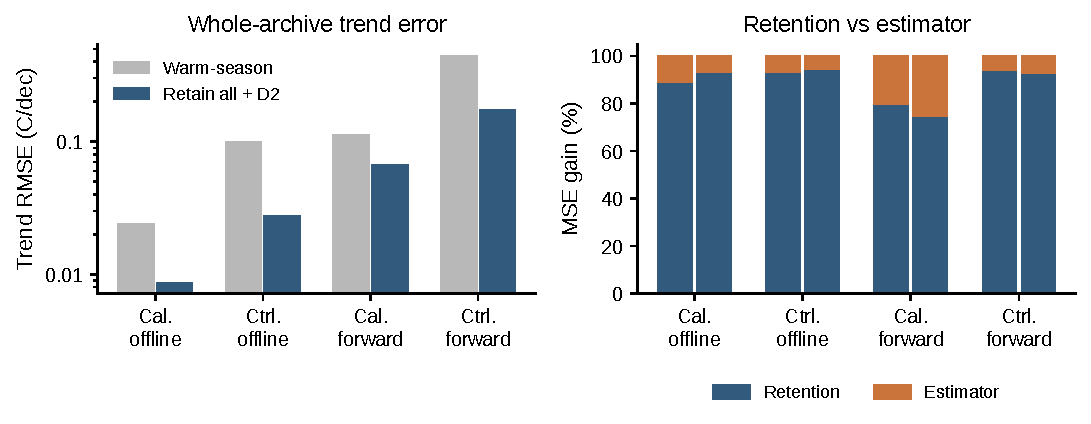
\includegraphics[width=\linewidth]{../wrr_tr/figures/simple_research/03_archive_factorial.pdf}
\caption{Whole-archive trend error and the retention/estimator decomposition. Left: trend RMSE on common station-repetition rows for warm-season screening and all-year recovery under D2, with archive and station/group counts. Right: percentage MSE gain from retention and estimator changes; paired bars use each method's own four-cell count. Takeaway: all-year recovery lowers the absolute slope error in 630 of 805 controlled-gap archives, raises it in 169 and leaves 6 numerically unchanged, so the aggregate gain is not universal.}
\label{fig:trend}
\end{figure}

\begin{figure}[t]
\centering
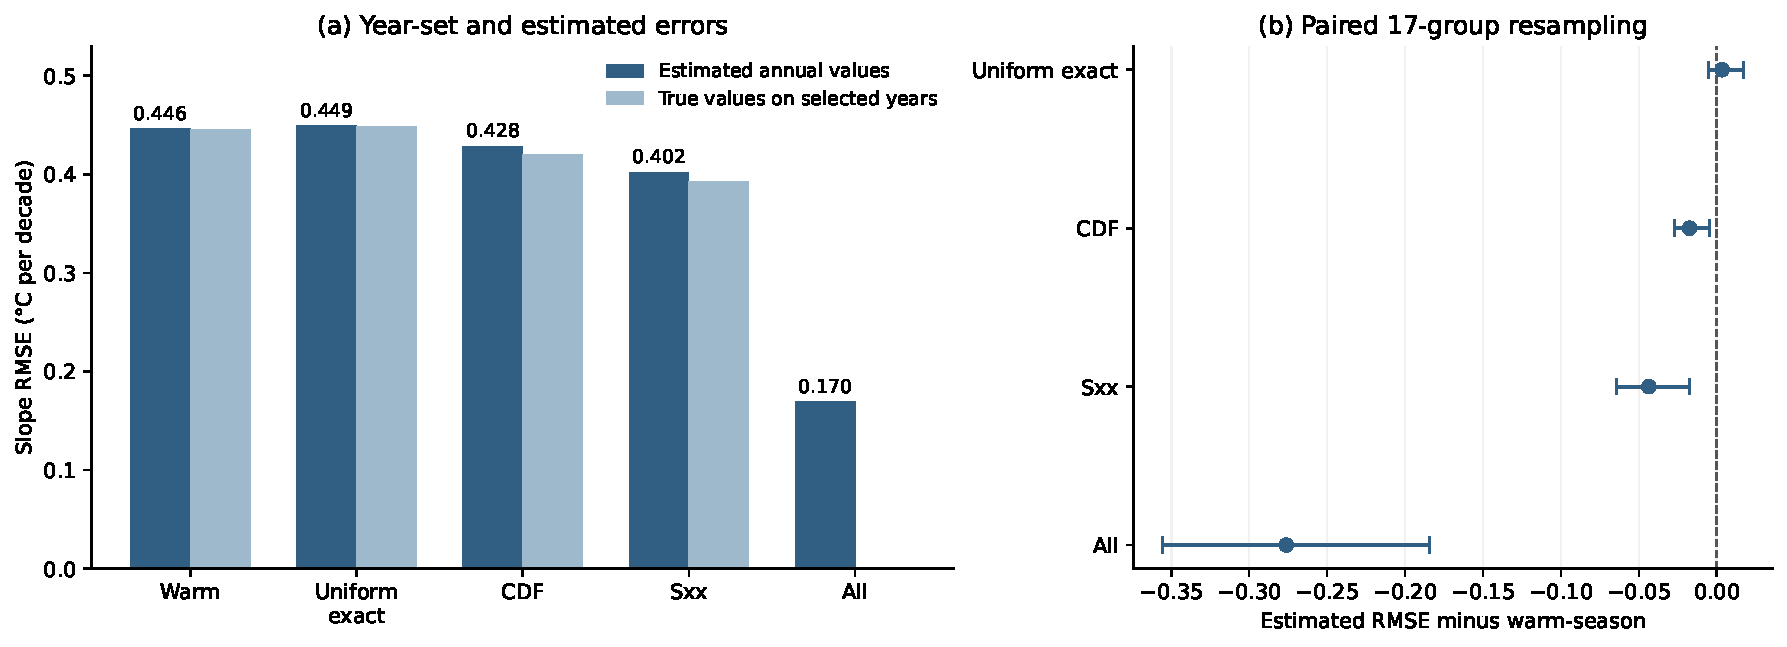
\includegraphics[width=\linewidth]{../wrr_tr/figures/process_revision/03_time_support.pdf}
\caption{Fixed-count year selection on 805 controlled-gap archives. Left: slope RMSE for warm-season screening, uniform exact subset averaging, CDF and $S_{xx}$ selection, using estimated annual values and complete-year H30 on the same selected years; all-year recovery is the reference. Right: comparator-minus-warm-season RMSE differences with paired 95\% percentile intervals from 10{,}000 resamples of 17 connected groups. Takeaway: CDF and $S_{xx}$ improve on warm-season screening at a fixed count, but all-year recovery remains closer to the complete-record slope (0.170 versus 0.428 and 0.402\,$^{\circ}$C/10a).}
\label{fig:selection}
\end{figure}

\begin{figure}[t]
\centering
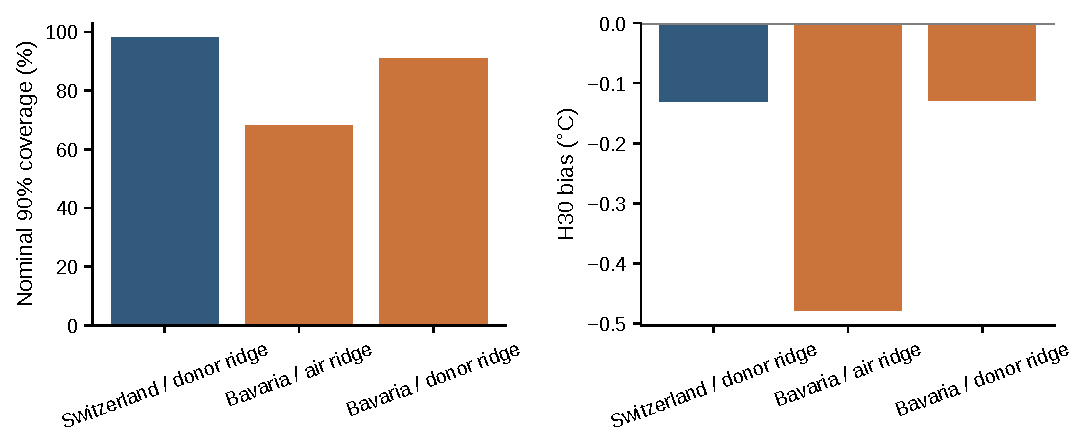
\includegraphics[width=\linewidth]{../wrr_tr/figures/process_revision/02_region_recovery.pdf}
\caption{Hidden-peak recovery by region and daily reconstructor. Left: nominal 90\% interval coverage; right: median bias (recovered minus complete-year H30). Bavarian air-ridge intervals cover 67.9\% of hidden peaks with a $-0.479$\,$^{\circ}$C bias, versus 90.8\% (Bavaria) and 98.1\% (Switzerland) for donor ridges; cases are not matched across reconstructors. Takeaway: recovery fails where local water information is absent, not merely where the calendar rule is imperfect.}
\label{fig:failure}
\end{figure}

\begin{figure}[t]
\centering
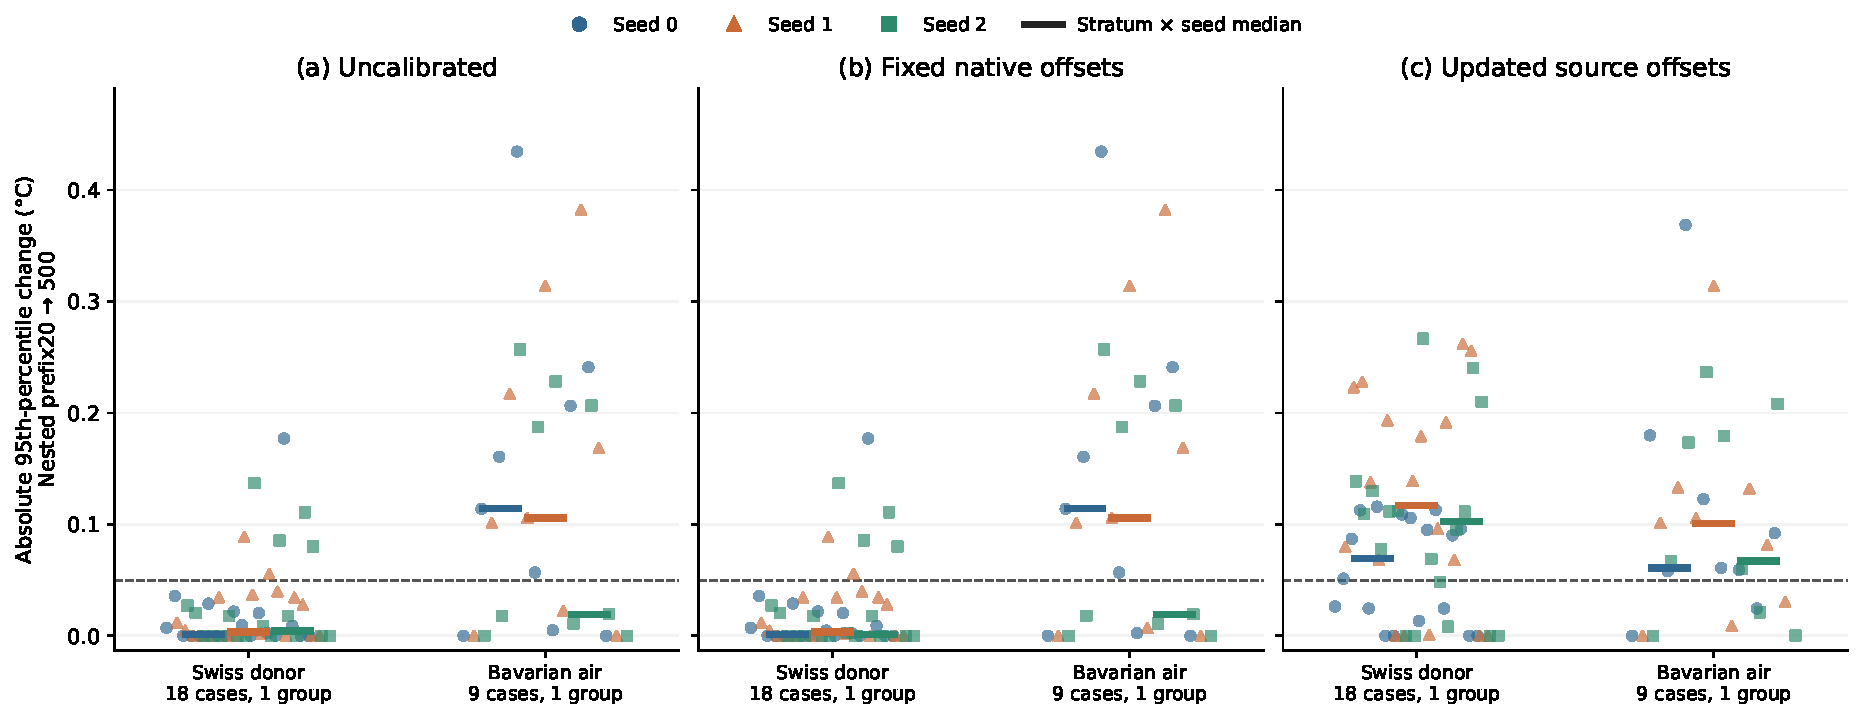
\includegraphics[width=\linewidth]{../wrr_tr/figures/process_revision/04_trajectory_budget.pdf}
\caption{Numerical sensitivity to the residual-bridge budget. Absolute change in the 95th-percentile endpoint between nested 20- and 500-path runs for the same 27 target cases under uncalibrated, fixed-offset and re-estimated-offset settings; colors are seeds and horizontal marks are stratum medians. The 0.05\,$^{\circ}$C line is a numerical diagnostic. Takeaway: the 20-path budget is a numerical-error floor; 500 paths on two target groups establish neither convergence nor a preferred estimator.}
\label{fig:budget}
\end{figure}
}{}
  \IfFileExists{open_source_flow.tex}{\subsection{Open-source model sensitivity}
A practical question for reuse is whether the comparison survives replacement of the restricted source providers by openly available products. As a candidate route, we refitted the source models on seven candidate providers with recorded reuse paths while retaining the target masks, daily features and plug-in baselines. On the crossed/forward cohort, the D2 trend RMSE changes from 0.164 to 0.158 $^{\circ}$C per decade and the classical RMSE from 0.147 to 0.156, over 738 four-way common pairs in 17 groups. The D2 retention fraction in the symmetric MSE decomposition falls from 93.9\% to 93.7\% on 807 factor cases, and nominal 95\% D2 interval coverage from 88.0\% to 87.6\% on 820 coverage cases. The substantive conclusions are unchanged. This is a candidate open reproducibility route, not a legal clearance: LUBW rights and the provenance of neighbour records still require confirmation. The candidate-source tables are descriptive, repetitions are not independent climates, and the filtered inputs remain processed study data rather than provider-native records. Global water-temperature modelling \citep{vanvliet2011} and recent assessments of water-temperature data coverage \citep{diaz2025} make such a route plausible, but its legal and operational status is not established here.

\subsection{Flow proxy diagnostic}
Flow can modify river thermal response \citep{vanvliet2011}, process models use discharge explicitly \citep{toffolon2015}, and regulated or groundwater-influenced reaches can change interval performance \citep{diaz2025}. Our evidence is diagnostic and associational. In the 336-station, 6,479-station-year USGS missingness sample, 21 stations in 17 groups recorded at least one zero-flow day and 16 stations in 14 groups recorded at least 30. A station-fixed conditional logit related a warm-season-incomplete year (the hidden-peak condition) to within-station standardized summer air temperature, within-station standardized summer log flow and a linear trend (per decade). In the flow-adjusted model, the odds ratio for the flow term is 0.594 [0.409, 0.813] for the recorded-zero cohort (282 station-years, 129 events) and 0.474 [0.265, 0.676] for the at-least-30-zero-day cohort (215 station-years, 104 events). Air temperature is 0.993 [0.659, 1.305] and 0.855 [0.580, 1.275]; the trend term is 1.198 [0.520, 1.883] and 1.292 [0.597, 2.132]. In the large fewer-than-30-zero-day cohort the flow odds ratio is 0.969 [0.897, 1.046]. The lower hidden-peak odds is an association in this proxy cohort, not evidence that low flow protects against underestimation. Zero flow is a historical proxy: no recorded zero does not prove perennial flow, and a zero does not identify an intermittent river, sensor exposure or a dry bed. The flow-adjusted subsets are smaller, so differences from the air-only model are not a mediation estimate.

The opened flow-comparator experiment provides a separate, non-causal check. It contains 255 sites, 8,999 complete climatic years and 134,925 cases; paired comparisons cover 210 sites, while the full 255-site cohort spans 17 HUC2 region groups. Historical D2 and single-donor Ridge baselines are already available. Donor-dependent methods are available on 81.7\% of crossed/all eligible cases versus 100\% for historical D2, and they do not lower paired mean absolute error (MAE; Table~\ref{tab:ems_flow_comparators}). In the danger scope, MOVE.1 has MAE 0.1062, the stochastic bridge 0.1038, single-donor Ridge 0.0896 and historical D2 0.0745. The flow comparators therefore show no accuracy gain here, and their lower availability is material.

\begin{table}[t]
\centering\footnotesize
\caption{Paired log-flow MAE in the opened flow-comparator cohort, crossed/all scope (66,099 common cases, 210 sites; the 255-site cohort spans 17 HUC2 region groups). ``Not worse'' is the percentage of sites where the left estimator's MAE does not exceed the right estimator's.}
\label{tab:ems_flow_comparators}
\resizebox{\linewidth}{!}{%
\begin{tabular}{lrrr}
\toprule
Comparison & Left MAE & Right MAE & Not worse (\%)\\
\midrule
MOVE.1 vs single-donor Ridge & 0.0734 & 0.0602 & 15.2\\
MOVE.1 vs historical D2 & 0.0734 & 0.0495 & 13.3\\
Stochastic bridge vs historical D2 & 0.0716 & 0.0495 & 28.1\\
\bottomrule
\end{tabular}}
\end{table}

The limitations are explicit: the zero-flow class is a station-level proxy; no 34-station FOEN/GKD daily flow merge was performed; air2stream-8 was not retrained with flow; no causal mechanism is identified; and rights and coverage for the required flow data remain unresolved. The comparator experiment is one opened positive-flow perennial subset, not a new blind transfer or a 20-seed stability claim.
}{}
}

\section*{Software and data availability}

\subsection*{Software}

\noindent\textbf{Software name:} \texttt{gapbench}, version 1.2.0.\\
\textbf{Developers:} [AUTHOR TO CONFIRM].\\
\textbf{Support:} public issue tracker and documentation in the repository.\\
\textbf{Year first available:} 2026.\\
\textbf{Hardware required:} Standard x86-64 workstation or laptop. Measured on one CPU core: the quickstart finishes in 0.13\,s with a peak resident set of 35\,MiB, and the full packaged replay of all 1{,}623 archive-level gap masks (8{,}115 retained-year strategy rows) finishes in 9.7\,s with a peak resident set of 289\,MiB.\\
\textbf{Software required:} Python $\ge$ 3.10, NumPy $\ge$ 1.24, and pandas $\ge$ 2.0; pytest $\ge$ 8 for the test suite.\\
\textbf{Program language:} Python.\\
\textbf{Program size:} 24 files, 1{,}012 lines of Python, 264\,KiB uncompressed (23\,KiB zipped, excluding caches).\\
\textbf{Availability:} Public repository, \url{https://github.com/shutiao23/stream-recoverability}, with code release v1.2.0 at \url{https://github.com/shutiao23/stream-recoverability/releases/tag/v1.2.0}; archival DOI [PENDING]. Reviewers can access the public repository without credentials.\\
\textbf{License:} MIT for code.\\
\textbf{Cost:} Free.\\
\textbf{30-minute quickstart:} From the repository root, run \texttt{pip install -e gapbench} and then \texttt{python gapbench/examples/quickstart.py}. The example builds a synthetic 20-year daily series with gaps, selects years under calendar-only rules, and decomposes finite-record slope error.

\subsection*{Data}

\textbf{Data sources:} Daily water-temperature records from FOEN (Switzerland), GKD Bayern (Bavaria), and USGS NWIS (United States), together with the additional providers documented in the manuscript; meteorological forcing from NASA POWER. Each provider's terms and attribution requirements apply.

\textbf{Restricted data:} LUBW records are subject to provider restrictions. The reviewer access route is being arranged with the provider and requires editorial and legal confirmation.

\noindent [EDITORIAL/LEGAL CONFIRMATION REQUIRED]

\textbf{Processed data:} Processed annual tables needed to reproduce the figures and trend summaries are included in the public repository. These tables contain derived annual quantities, not the restricted daily observations.

\textbf{Archival identifiers:} DOIs for the archived code release and processed tables are [PENDING].

\textbf{Code versus data rights:} The MIT license applies to the \texttt{gapbench} code. It does not relicense observational data, which remain subject to the terms of FOEN, GKD Bayern, USGS, LUBW, NASA POWER, and other providers. Code availability does not imply redistribution rights for provider data.

\section*{CRediT authorship contribution statement}

\noindent\textbf{Conceptualization:} [AUTHOR TO CONFIRM].\\
\textbf{Methodology:} [AUTHOR TO CONFIRM].\\
\textbf{Software:} [AUTHOR TO CONFIRM].\\
\textbf{Validation:} [AUTHOR TO CONFIRM].\\
\textbf{Formal analysis:} [AUTHOR TO CONFIRM].\\
\textbf{Investigation:} [AUTHOR TO CONFIRM].\\
\textbf{Data curation:} [AUTHOR TO CONFIRM].\\
\textbf{Writing -- original draft:} [AUTHOR TO CONFIRM].\\
\textbf{Writing -- review and editing:} [AUTHOR TO CONFIRM].\\
\textbf{Visualization:} [AUTHOR TO CONFIRM].\\
\textbf{Supervision:} [AUTHOR TO CONFIRM].\\
\textbf{Funding acquisition:} [AUTHOR TO CONFIRM].

\section*{Declaration of competing interest}

The authors declare that they have no known competing financial interests or personal relationships that could have appeared to influence the work reported in this paper. [AUTHOR TO CONFIRM]

\section*{Funding}

[Funding sources and grant numbers, or a statement that no specific funding was received.] [AUTHOR TO CONFIRM]

\section*{Ethics and data statement}

No human participants or animals were involved. Observational river-temperature and meteorological records were obtained from the providers listed in the Software and Data Availability statement and used under their respective terms. Access to restricted LUBW records is described there; the final permissions wording requires editorial and legal confirmation.

\noindent [EDITORIAL/LEGAL CONFIRMATION REQUIRED]

\section*{Declaration of generative AI and AI-assisted technologies}

During the preparation of this work the authors used AI-assisted coding and editing tools, including Cursor, to support code development, consistency checks, and language editing. After using these tools, the authors reviewed and edited all content, verified all scientific claims and results, and take full responsibility for the content of the publication. [AUTHOR TO CONFIRM]


\bibliographystyle{elsarticle-harv}
\bibliography{references_ems}

\end{document}
